\section{COMBO Proofs from Section~\ref{sec:combo_theory}}
\label{app:combo_proofs}

In this section, we provide proofs for theoretical results in Section~\ref{sec:combo_theory}. Before the proofs, we note that all statements are proven in the case of finite state space (i.e., $|\states| < \infty$) and finite action space (i.e., $|\actions| < \infty$) we define some commonly appearing notation symbols appearing in the proof: 
\begin{itemize}
\vspace{-5pt}
    \item $P_{\mdp}$ and $r_{\mdp}$ (or $P$ and $r$ with no subscript for notational simplicity) denote the dynamics and reward function of the actual MDP $\mdp$
    \vspace{-5pt}
    \item $P_{\mdpbar}$ and $r_{\mdpbar}$ denote the dynamics and reward of the empirical MDP $\mdpbar$ generated from the transitions in the dataset
    \vspace{-5pt}
    \item $P_{\mdphat}$ and $r_{\mdphat}$ denote the dynamics and reward of the MDP induced by the learned model $\mdphat$
\end{itemize}
\vspace{-5pt}
We also assume that whenever the cardinality of a particular state or state-action pair in the offline dataset $\data$, denoted by $|\mathcal{D}(\bs, \mathbf{a})|$, appears in the denominator, we assume it is non-zero. For any non-existent $(\bs, \mathbf{a}) \notin \data$, we can simply set $|\data(\bs, \mathbf{a})|$ to be a small value $< 1$, which prevents any bound from producing trivially $\infty$ values.

\subsection{A Useful Lemma and Its Proof}
\label{app:proof_lemma}

Before proving our main results, we first show that the penalty
term in equation \ref{eqn:combo_iterate} is positive in expectation. Such a positive penalty is important to combat any overestimation that may
arise as a result of using $\bellmanhat$.

\begin{lemma}[(Interpolation Lemma]
\label{thm:line_thm}
For any $f \in [0, 1]$, and any given $\rho(\bs, \mathbf{a}) \in \Delta^{|\states||\actions|}$, let $d_f$ be an f-interpolation of $\rho$ and $\data$, i.e., $d_f(\bs, \mathbf{a}) := f d(\bs, \mathbf{a}) + (1-f) \rho(\bs, \mathbf{a})$. For a given iteration $k$ of Equation~\ref{eqn:combo_iterate}, we restate the definition of the expected penalty under $\rho(\bs, \mathbf{a})$ in Eq.~\ref{eqn:expected_penalty}: 
\begin{equation*}
 \nu(\rho, f) := \E_{\bs, \mathbf{a} \sim \rho(\bs, \mathbf{a})}\left[\frac{\rho(\bs, \mathbf{a}) - d(\bs, \mathbf{a})}{d_f(\bs, \mathbf{a})} \right].
\end{equation*}
Then $\nu(\rho, f)$ satisfies, (1) $\nu(\rho, f) \geq 0,~~ \forall \rho, f$, (2) $\nu(\rho, f)$ is monotonically increasing in $f$ for a fixed $\rho$, and (3) $\nu(\rho, f) = 0$ iff $\forall~ \bs, \mathbf{a}, ~\rho(\bs, \mathbf{a}) = d(\bs, \mathbf{a}) \text{~or~} f = 0$. 
\end{lemma}
\begin{proof}
To prove this lemma, we use algebraic manipulation on the expression for quantity $\nu(\rho, f)$ and show that it is indeed positive and monotonically increasing in $f \in [0, 1]$.
\begin{align}
    \nu(\rho, f) &= \sum_{\bs, \mathbf{a}} \rho(\bs, \mathbf{a}) \left(\frac{\rho(\bs, \mathbf{a}) - d(\bs, \mathbf{a})}{f d(\bs, \mathbf{a}) + (1 - f) \rho(\bs, \mathbf{a})}\right)\nonumber \\
    &= \sum_{\bs, \mathbf{a}} \rho(\bs, \mathbf{a}) \left(\frac{\rho(\bs, \mathbf{a}) - d(\bs, \mathbf{a})}{\rho(\bs, \mathbf{a}) + f ( d(\bs, \mathbf{a}) - \rho(\bs, \mathbf{a}))}\right)\\
    \implies \frac{d \nu(\rho, f)}{d f} &= \sum_{\bs, \mathbf{a}} \rho(\bs, \mathbf{a}) \left(\rho(\bs, \mathbf{a}) - d(\bs, \mathbf{a})\right)^2 \cdot \left(\frac{1}{(\rho(\bs, \mathbf{a}) + f ( d(\bs, \mathbf{a}) - \rho(\bs, \mathbf{a}))}\right)^2 \geq 0\nonumber\\
    &~~~\forall f \in [0, 1].
\end{align}
Since the derivative of $\nu(\rho, f)$ with respect to $f$ is always positive, it is an increasing function of $f$ for a fixed $\rho$, and this proves the second part (2) of the Lemma. Using this property, we can show the part (1) of the Lemma as follows:
\begin{align}
    \forall f \in (0, 1],~ \nu(\rho, f) \geq \nu(\rho, 0) = \sum_{\bs, \mathbf{a}} \rho(\bs, \mathbf{a}) \frac{\rho(\bs, \mathbf{a}) - d(\bs, \mathbf{a})}{\rho(\bs, \mathbf{a})} &= \sum_{\bs, \mathbf{a}} \left( \rho(\bs, \mathbf{a}) - d(\bs, \mathbf{a}) \right)\nonumber\\
    &= 1 - 1 = 0.
\end{align}
Finally, to prove the third part (3) of this Lemma, note that when $f = 0$, $\nu(\rho, f) = 0$ (as shown above), and similarly by setting $\rho(\bs, \mathbf{a}) = d(\bs, \mathbf{a})$ note that we obtain $\nu(\rho, f) = 0$. To prove the only if side of (3), assume that $f \neq 0$ and $\rho(\bs, \mathbf{a}) \neq d(\bs, \mathbf{a})$ and we will show that in this case $\nu(\rho,f) \neq 0$. When $d(\bs, \mathbf{a}) \neq \rho(\bs, \mathbf{a})$, the derivative $\frac{d \nu(\rho,f)}{d f} > 0$ (i.e., strictly positive) and hence the function $\nu(\rho, f)$ is a strictly increasing function of $f$. Thus, in this case, $\nu(\rho, f) > 0 = \nu(\rho, 0)~ \forall f > 0$. Thus we have shown that if $\rho(\bs, \mathbf{a}) \neq d(\bs, \mathbf{a})$ and $f > 0$, $\nu(\rho, f) \neq 0$, which completes our proof for the only if side of (3). 
\end{proof}

\subsection{Proof of Proposition~\ref{thm:lower_bound}}
\label{app:proof_lower_bound}
Before proving this proposition, we provide a bound on the Bellman backup in the empirical MDP, $\bellman_{\mdpbar}$. To do so, we formally define the standard concentration properties of the reward and transition dynamics in the empirical MDP, $\mdpbar$, that we assume so as to prove Proposition~\ref{thm:line_thm}. Following prior work~\citep{osband2017posterior,jaksch2010near,kumar2020conservative}, we assume:
\begin{assumption}
\label{assumption:conc}
    $\forall~ \bs, \mathbf{a} \in \mdp$, the following relationships hold with high probability, $\geq 1 - \delta$
    \begin{equation*}
        |r_{\mdpbar}(\bs, \mathbf{a}) - r(\bs, \mathbf{a})| \leq \frac{C_{r, \delta}}{\sqrt{|\mathcal{D}(\bs, \mathbf{a})|}}, ~~~ ||P_{\mdpbar}(\bs'|\bs, \mathbf{a}) - P(\bs'|\bs, \mathbf{a})||_{1} \leq \frac{C_{P, \delta}}{\sqrt{|\mathcal{D}(\bs, \mathbf{a})|}}.
    \end{equation*}
\end{assumption}
Under this assumption and assuming that the reward function in the MDP, $r(\bs, \mathbf{a})$ is bounded, as $|r(\bs, \mathbf{a})| \leq R_{\max}$, we can bound the difference between the empirical Bellman operator, $\bellman_{\mdpbar}$ and the actual MDP, $\bellman_\mdp$,
\begin{align*}
    \left\vert\left({\bellman_{\mdpbar}}^\policy \hat{Q}^k \right) - \left({\bellman}^\policy_\mdp \hat{Q}^k \right)\right\vert &= \left\vert\left(r_{\mdpbar}(\bs, \mathbf{a}) - r_\mdp(\bs, \mathbf{a})\right)\right.\\
    &\left.+ \gamma \sum_{\bs'} \left({P}_{\mdpbar}(\bs'|\bs, \mathbf{a}) - P_\mdp(\bs'|\bs,\mathbf{a})\right) \E_{\policy(\mathbf{a}'|\bs')}\left[\hat{Q}^k(\bs' , \mathbf{a}')\right]\right\vert\\
    &\leq \left\vert r_{\mdpbar}(\bs, \mathbf{a}) - r_\mdp(\bs, \mathbf{a})\right\vert\\
    &+ \gamma \left\vert \sum_{\bs'} \left({P}_{\mdpbar}(\bs'|\bs, \mathbf{a}) - P_\mdp(\bs'|\bs,\mathbf{a})\right) \E_{\policy(\mathbf{a}'|\bs')}\left[\hat{Q}^k(\bs' , \mathbf{a}')\right]\right\vert\\
    &\leq \frac{C_{r, \delta} + \gamma C_{P, \delta} 2R_{\max} / (1 - \gamma)}{\sqrt{|\mathcal{D}(\bs, \mathbf{a})|}}. 
\end{align*}
Thus the overestimation due to sampling error in the empirical MDP, $\mdpbar$ is bounded as a function of a bigger constant, $C_{r, P, \delta}$ that can be expressed as a function of $C_{r, \delta}$ and $C_{P, \delta}$, and depends on $\delta$ via a $\sqrt{\log (1/\delta)}$ dependency. For the purposes of proving Proposition~\ref{thm:Q_bound}, we assume that:
\begin{equation}
\label{eqn:sampling_error}
    \forall \bs, \mathbf{a}, ~~\left\vert\left({\bellman_{\mdpbar}}^\policy \hat{Q}^k \right) - \left({\bellman}^\policy_\mdp \hat{Q}^k \right)\right\vert  \leq \frac{C_{r, T, \delta} R_{\max}}{(1 - \gamma) \sqrt{|\mathcal{D}(\bs, \mathbf{a})|}}.
\end{equation}

Next, we provide a bound on the error between the bellman backup induced by the learned dynamics model and the learned reward, $\bellman_{\mdphat}$, and the actual Bellman backup, $\bellman_{\mdp}$. To do so, we note that:
\begin{align}
    \left\vert\left({\bellman_{\mdphat}}^\policy \hat{Q}^k \right) - \left({\bellman}^\policy_\mdp \hat{Q}^k \right)\right\vert &= \left\vert\left(r_{\mdphat}(\bs, \mathbf{a}) - r_\mdp(\bs, \mathbf{a})\right)\right.\\
    &\left.+ \gamma \sum_{\bs'} \left({P}_{\mdphat}(\bs'|\bs, \mathbf{a}) - P_\mdp(\bs'|\bs,\mathbf{a})\right) \E_{\policy(\mathbf{a}'|\bs')}\left[\hat{Q}^k(\bs' , \mathbf{a}')\right]\right\vert \nonumber\\ 
    &\leq |r_{\mdphat}(\bs, \mathbf{a}) - r_\mdp(\bs, \mathbf{a})| + \gamma \frac{2 R_{\max}}{1 - \gamma} D(P, P_{\mdphat}),
    \label{eqn:model_error} 
\end{align}
where $D(P, P_{\mdphat})$ is the total-variation divergence between the learned dynamics model and the actual MDP. Now, we show that the asymptotic Q-function learned by COMBO lower-bounds the actual Q-function of any
policy $\pi$ with high probability for a large enough $\beta \geq 0$. We will use Equations~\ref{eqn:sampling_error} and \ref{eqn:model_error} to prove such a result.

\begin{proposition}[Asymptotic lower-bound]
\label{thm:Q_bound}
Let $P^\pi$ denote the Hadamard product of the dynamics $P$ and a given policy $\pi$ in the actual MDP and let $S^\pi := (I - \gamma P^\pi)^{-1}$. Let $D$ denote the total-variation divergence between two probability distributions. For any $\pi(\mathbf{a}|\bs)$, the Q-function obtained by recursively applying Equation~\ref{eqn:combo_iterate}, with $\hat{{\bellman}}^\pi = f \bellman_{\mdpbar}^\pi + (1 - f) \bellman_{\mdphat}^\pi$, with probability at least $1 - \delta$, results in $\hat{Q}^\pi$ that satisfies:
\begin{align*}
    \forall \bs, \mathbf{a},~ \hat{Q}^\pi(\bs, \mathbf{a}) \leq  Q^\pi(\bs, \mathbf{a}) &- \beta \cdot \left[ S^\pi \left[ \frac{\rho - d}{d_f} \right] \right](\bs, \mathbf{a}) + f \left[ S^\pi \left[ \frac{C_{r, T, \delta} R_{\max}}{(1 - \gamma) \sqrt{|\data|}} \right] \right](\bs, \mathbf{a})\\
    +&~ (1 - f) \left[ S^\pi \left[ |r - r_{\mdphat}| + \frac{ 2 \gamma  R_{\max}}{1 - \gamma} D(P, P_{\mdphat}) \right]  \right]\!\! (\bs, \mathbf{a}).
\end{align*}
\end{proposition}
\begin{proof}
We first note that the Bellman backup $\hat{\bellman}^\pi$ induces the following Q-function iterates as per Equation~\ref{eqn:combo_iterate},
\begin{align*}
    \hat{Q}^{k+1}(\bs, \mathbf{a}) &= \left(\hat{\bellman}^\pi \hat{Q}^k\right)(\bs, \mathbf{a}) - \beta \frac{\rho(\bs, \mathbf{a}) - d(\bs, \mathbf{a})}{d_f(\bs, \mathbf{a})}\\
    &=  f \left(\bellman^\pi_{\mdpbar} \hat{Q}^k \right) (\bs, \mathbf{a}) + (1 - f) \left(\bellman^\pi_{\mdphat} \hat{Q}^k \right) (\bs, \mathbf{a}) - \beta \frac{\rho(\bs, \mathbf{a}) - d(\bs, \mathbf{a})}{d_f(\bs, \mathbf{a})}\\
    &= \left(\bellman^\pi \hat{Q}^k\right)(\bs, \mathbf{a}) - \beta \frac{\rho(\bs, \mathbf{a}) - d(\bs, \mathbf{a})}{d_f(\bs, \mathbf{a})} + (1 - f) \left({\bellman_{\mdphat}}^\policy \hat{Q}^k - {\bellman}^\policy \hat{Q}^k \right)(\bs, \mathbf{a})\\
    &+ f  \left({\bellman_{\mdpbar}}^\policy \hat{Q}^k - {\bellman}^\policy \hat{Q}^k \right)(\bs, \mathbf{a})\\
   \forall \bs, \mathbf{a},~ \hat{Q}^{k+1} &\leq \left(\bellman^\pi \hat{Q}^k\right) - \beta \frac{\rho - d}{d_f} + (1 - f) \left[|r_{\mdphat} - r_\mdp| + \frac{2 \gamma R_{\max}}{1 - \gamma} D(P, P_{\mdphat}) \right] + f \frac{C_{r, T, \delta} R_{\max}}{(1 - \gamma) \sqrt{|\data|}} 
\end{align*}
Since the RHS upper bounds the Q-function pointwise for each $(\bs, \mathbf{a})$, the fixed point of the Bellman iteration process will be pointwise smaller than the fixed point of the Q-function found by solving for the RHS via equality. Thus, we get that
\begin{align*}
    \hat{Q}^\pi(\bs, \mathbf{a}) &\leq \underbrace{ S^\pi r_{\mdp}}_{= Q^\pi(\bs, \mathbf{a})} -\beta \left[ S^\pi \left[ \frac{\rho - d}{d_f} \right] \right](\bs, \mathbf{a}) +~ f \left[ S^\pi \left[ \frac{C_{r, T, \delta} R_{\max}}{(1 - \gamma) \sqrt{|\data|}} \right] \right](\bs, \mathbf{a})\\
    &+~ (1 - f) \left[ S^\pi \left[ |r - r_{\mdphat}| + \frac{ 2 \gamma  R_{\max}}{1 - \gamma} D(P, P_{\mdphat}) \right]  \right]\!\! (\bs, \mathbf{a}),  
\end{align*}
which completes the proof of this proposition.
\end{proof}

Next, we use the result and proof technique from Proposition~\ref{thm:Q_bound} to prove Corollary~\ref{thm:lower_bound}, that in expectation under the initial state-distribution, the expected Q-value is indeed a lower-bound. 

\begin{corollary}[Corollary~\ref{thm:lower_bound} restated]
For a sufficiently large $\beta$, we have a lower-bound that
$\E_{\bs \sim \mu_0, \mathbf{a} \sim \policy(\cdot|\bs)}[\hat{Q}^\pi(\bs, \mathbf{a})] \leq \E_{\bs \sim \mu_0, \mathbf{a} \sim \policy(\cdot|\bs)}[Q^\pi(\bs, \mathbf{a})]$, 
where $\mu_0(\bs)$ is the initial state distribution. 
Furthermore, when $\epsilon_{\text{s}}$ is small, such as in the large sample regime; or when the model bias $\epsilon_{\text{m}}$ is small, a small $\beta$ is sufficient along with an appropriate choice of $f$.
\end{corollary}

\begin{proof}
To prove this corollary, we note a slightly different variant of Proposition~\ref{thm:Q_bound}. To observe this, we will deviate from the proof of Proposition~\ref{thm:Q_bound} slightly and will aim to express the inequality using $\bellman_{\mdphat}$, the Bellman operator defined by the learned model and the reward function. Denoting $(I - \gamma P_{\mdphat})^{-1}$ as $S_{\mdphat}^\pi$, doing this will intuitively allow us to obtain $\beta \left(\mu(\bs) \policy(\mathbf{a}|\bs)\right)^T \left(S_{\mdphat}^\pi \left[\frac{\rho - d}{d_f} \right]\right)(\bs, \mathbf{a})$ as the conservative penalty which can be controlled by choosing $\beta$ appropriately so as to nullify the potential overestimation caused due to other terms. Formally,
\begin{align*}
    \hat{Q}^{k+1}(\bs, \mathbf{a}) &= \left(\hat{\bellman}^\pi \hat{Q}^k\right)(\bs, \mathbf{a}) - \beta \frac{\rho(\bs, \mathbf{a}) - d(\bs, \mathbf{a})}{d_f(\bs, \mathbf{a})} = \left(\bellman^\pi_{\mdphat} \hat{Q}^k \right)(\bs, \mathbf{a}) -  \beta \frac{\rho(\bs, \mathbf{a}) - d(\bs, \mathbf{a})}{d_f(\bs, \mathbf{a})}\\
    &+ f \underbrace{\left(\bellman^\pi_{\mdpbar} - \bellman^\pi_{\mdphat} \hat{Q}^k \right)(\bs, \mathbf{a})}_{:= \Delta(\bs, \mathbf{a})}
\end{align*}
By controlling $\Delta(\bs, \mathbf{a})$ using the pointwise triangle inequality:
\begin{equation}
    \forall \bs, \mathbf{a}, ~\left\vert \bellman^\pi_{\mdpbar} \hat{Q}^k - \bellman^\pi_{\mdphat} \hat{Q}^k \right\vert \leq \left\vert \bellman^\pi \hat{Q}^k - \bellman^\pi_{\mdphat} \hat{Q}^k \right\vert + \left\vert \bellman^\pi_{\mdpbar} \hat{Q}^k - \bellman^\pi \hat{Q}^k \right\vert,
\end{equation}
and then iterating the backup $\bellman^\pi_{\mdphat}$ to its fixed point and finally noting that $\rho(\bs, \mathbf{a}) = \left((\mu \cdot \pi)^T S^\pi_{\mdphat}\right)(\bs, \mathbf{a})$, we obtain:
\begin{equation}
    \E_{\mu, \pi}[\hat{Q}^\pi(\bs, \mathbf{a})] \leq \E_{\mu, \pi}[Q^\pi_{\mdphat}(\bs, \mathbf{a})] - \beta~ \E_{\rho(\bs, \mathbf{a})}\left[\frac{\rho(\bs, \mathbf{a}) - d(\bs, \mathbf{a})}{d_f(\bs, \mathbf{a})}\right] + \mathrm{terms~ independent~ of~} \beta.
\end{equation}
%%AK: there is one more term in the equation above, fit it in one line...
The terms marked as ``terms independent of $\beta$'' correspond to the additional positive error terms obtained by iterating $\left\vert \bellman^\pi \hat{Q}^k - \bellman^\pi_{\mdphat} \hat{Q}^k \right\vert$ and $\left\vert \bellman^\pi_{\mdpbar} \hat{Q}^k - \bellman^\pi \hat{Q}^k \right\vert$, which can be bounded similar to the proof of Proposition~\ref{thm:Q_bound} above. Now by replacing the model Q-function, $\E_{\mu, \pi}[Q^\pi_{\mdphat}(\bs, \mathbf{a})]$ with the actual Q-function, $\E_{\mu, \pi}[Q^\pi(\bs, \mathbf{a})]$ and adding an error term corresponding to model error to the bound, we obtain that:
\begin{equation}
\label{eqn:lower_bound_eqn}
    \E_{\mu, \pi}[\hat{Q}^\pi(\bs, \mathbf{a})] \leq \E_{\mu, \pi}[Q^\pi(\bs, \mathbf{a})] + \mathrm{terms~ independent~ of~} \beta - \beta~ \underbrace{\E_{\rho(\bs, \mathbf{a})}\left[\frac{\rho(\bs, \mathbf{a}) - d(\bs, \mathbf{a})}{d_f(\bs, \mathbf{a})}\right]}_{= \nu(\rho, f) > 0}.
\end{equation}
Hence, by choosing $\beta$ large enough, we obtain the desired lower bound guarantee. 
\end{proof}

\begin{remark}[\underline{\textbf{COMBO does not underestimate at every $\bs \in \mathcal{D}$ unlike CQL.}}]
\label{remak:tighter_lower_bound}
Before concluding this section, we discuss how the bound obtained by COMBO (Equation~\ref{eqn:lower_bound_eqn}) is tighter than CQL. CQL learns a Q-function such that the value of the policy under the resulting Q-function lower-bounds the true value function at each state $\bs \in \mathcal{D}$ individually (in the absence of no sampling error), i.e., $\forall \bs \in \mathcal{D}, \hat{V}^\pi_{\text{CQL}}(\bs) \leq V^\pi(\bs)$, whereas the bound in COMBO is only valid in expectation of the value function over the initial state distribution, i.e., $\E_{\bs \sim \mu_0(\bs)}[\hat{V}^\pi_{\text{COMBO}}(\bs)] \leq \E_{\bs \sim \mu_0(\bs)}[V^\pi(\bs)]$, and the value function at a given state may not be a lower-bound. For instance, COMBO can overestimate the value of a state more frequent in the dataset distribution $d(\bs, \mathbf{a})$ but not so frequent in the $\rho(\bs, \mathbf{a})$ marginal distribution of the policy under the learned model $\mdphat$. To see this more formally, note that the expected penalty added in the effective Bellman backup performed by COMBO (Equation~\ref{eqn:combo_iterate}), in expectation under the dataset distribution $d(\bs, \mathbf{a})$, $\widetilde{\nu}(\rho, d, f)$ is actually \textbf{\textit{negative}}:
\begin{align*}
    \widetilde{\nu}(\rho, d, f) = \sum_{\bs, \mathbf{a}} d(\bs, \mathbf{a}) \frac{\rho(\bs, \mathbf{a}) - d(\bs, \mathbf{a})}{d_f(\bs, \mathbf{a})} = - \sum_{\bs, \mathbf{a}} d(\bs, \mathbf{a}) \frac{d(\bs, \mathbf{a}) - \rho(\bs, \mathbf{a})}{f d(\bs, \mathbf{a}) + (1 - f) \rho(\bs, \mathbf{a})} < 0,
\end{align*}
where the final inequality follows via a direct application of the proof of Lemma~\ref{thm:line_thm}. Thus, COMBO actually \emph{overestimates} the values at atleast some states (in the dataset) unlike CQL.   
\end{remark}

\subsection{Proof of Proposition~\ref{prop:less_conservative}}
\label{app:proof_less_conservative}

In this section, we will provide a proof for Proposition~\ref{prop:less_conservative}, and show that the COMBO can be less conservative in terms of the estimated value. To recall, let $\Delta^\pi_\text{COMBO} := \E_{\bs, \mathbf{a} \sim d_{\mdpbar}(\bs), \pi(\mathbf{a}|\bs)}\left[\hat{Q}^\pi(\bs, \mathbf{a} \right]$ and let $\Delta^\pi_\text{CQL} := \E_{\bs, \mathbf{a} \sim d_{\mdpbar}, \pi(\mathbf{a}|\bs)} \left[\hat{Q}^\pi_\text{CQL}(\bs, \mathbf{a}) \right]$. From \citet{kumar2020conservative}, we obtain that $\hat{Q}^\pi_\text{CQL}(\bs, \mathbf{a}) := Q^\pi(\bs, \mathbf{a}) - \beta \frac{\pi(\mathbf{a}|\bs) - \pi_\beta(\mathbf{a}|\bs)}{\pi_\beta(\mathbf{a}|\bs)}$. We shall derive the condition for the real data fraction $f=1$ for COMBO, thus making sure that $d_f(\bs) = d^{\pi_\beta}(\bs)$. To derive the condition when $\Delta^\pi_\text{COMBO} \geq \Delta^\pi_\text{CQL}$, we note the following simplifications:
\begin{align}
    & \Delta^\pi_\text{COMBO} \geq \Delta^\pi_\text{CQL} \\
    \implies & \sum_{\bs, \mathbf{a}} d_{\mdpbar}(\bs) \pi(\mathbf{a}|\bs) \hat{Q}^\pi(\bs, \mathbf{a}) \geq \sum_{\bs, \mathbf{a}} d_{\mdpbar}(\bs) \pi(\mathbf{a}|\bs) \hat{Q}^\pi_\text{CQL}(\bs, \mathbf{a}) \\
    \label{eqn:cql_vs_combo_terms}
    \implies & \beta \sum_{\bs, \mathbf{a}} d_{\mdpbar}(\bs)\pi(\mathbf{a}|\bs) \left( \frac{\rho(\bs, \mathbf{a}) - d^{\pi_\beta}(\bs) \pi_\beta(\mathbf{a}|\bs)}{d^{\pi_\beta}(\bs) \pi_\beta(\mathbf{a}|\bs)} \right) \leq \beta \sum_{\bs, \mathbf{a}} d_{\mdpbar}(\bs)\pi(\mathbf{a}|\bs) \left(\frac{\pi(\mathbf{a}|\bs) - \pi_\beta(\mathbf{a}|\bs)}{\pi_\beta(\mathbf{a}|\bs)} \right).
\end{align}
Now, in the expression on the left-hand side, we add and subtract $d^{\pi_\beta}(\bs) \pi(\mathbf{a}|\bs)$ from the numerator inside the paranthesis.
\begin{align}
    & \sum_{\bs, \mathbf{a}} d_{\mdpbar}(\bs, \mathbf{a}) \left( \frac{\rho(\bs, \mathbf{a}) - d^{\pi_\beta}(\bs) \pi_\beta(\mathbf{a}|\bs)}{d^{\pi_\beta}(\bs) \pi_\beta(\mathbf{a}|\bs)} \right)\\
    &= \sum_{\bs, \mathbf{a}} d_{\mdpbar}(\bs, \mathbf{a}) \left( \frac{\rho(\bs, \mathbf{a}) - d^{\pi_\beta}(\bs) \pi(\mathbf{a}|\bs) + d^{\pi_\beta}(\bs) \pi(\mathbf{a}|\bs) - d^{\pi_\beta}(\bs) \pi_\beta(\mathbf{a}|\bs)}{d^{\pi_\beta}(\bs) \pi_\beta(\mathbf{a}|\bs)} \right)\\
    &= \underbrace{\sum_{\bs, \mathbf{a}} d_{\mdpbar}(\bs, \mathbf{a}) \frac{\pi(\mathbf{a}|\bs) - \pi_\beta(\mathbf{a}|\bs)}{\pi_\beta(\mathbf{a}|\bs)}}_{(1)} + \sum_{\bs, \mathbf{a}} d_{\mdpbar}(\bs, \mathbf{a}) \cdot \frac{\rho(\bs) - d^{\pi_\beta}(\bs)}{d^{\pi_\beta}(\bs)} \cdot \frac{\pi(\mathbf{a}|\bs)}{\pi_\beta(\mathbf{a}|\bs)}
\end{align}
The term marked $(1)$ is identical to the CQL term that appears on the right in Equation~\ref{eqn:cql_vs_combo_terms}. Thus the inequality in Equation~\ref{eqn:cql_vs_combo_terms} is satisfied when the second term above is negative. To show this, first note that $d^{\pi_\beta}(\bs) = d_{\mdpbar}(\bs)$ which results in a cancellation. Finally, re-arranging the second term into expectations gives us the desired result. An analogous condition can be derived when $f \neq 1$, but we omit that derivation as it will be hard to interpret terms appear in the final inequality.

\subsection{Proof of Proposition~\ref{thm:policy_improvement}}
\label{app:proof_policy_improvement}

To prove the policy improvement result in Proposition~\ref{thm:policy_improvement}, we first observe that using Equation~\ref{eqn:combo_iterate} for Bellman backups amounts to finding a policy that maximizes the return of the policy in the a modified ``f-interpolant'' MDP which admits the Bellman backup $\bellmanhat^\pi$, and is induced by a linear interpolation of backups in the empirical MDP $\mdpbar$ and the MDP induced by a dynamics model $\mdphat$ and the return of a policy $\pi$ in this effective f-interpolant MDP is denoted by $J(\mdpbar, \mdphat, f, \pi)$. Alongside this, the return is penalized by the conservative penalty where $\rho^\pi$ denotes the marginal state-action distribution of policy $\pi$ in the learned model $\mdphat$. 
\begin{equation}
    \hat{J}(f, \pi) = J(\mdpbar, \mdphat, f, \pi)  - \beta \frac{\nu(\rho^\pi, f)}{1 - \gamma}.
\label{eqn:penalized_objective}
\end{equation}
We will require bounds on the return of a policy $\pi$ in this f-interpolant MDP, $J(\mdpbar, \mdphat, f, \pi)$, which we first prove separately as Lemma~\ref{lemma:interpolant_regular_bound} below and then move to the proof of Proposition~\ref{thm:policy_improvement}.

\begin{lemma}[Bound on return in f-interpolant MDP]
\label{lemma:interpolant_regular_bound}
For any two MDPs, $\mdp_1$ and $\mdp_2$, with the same state-space, action-space and discount factor, and for a given fraction $f \in [0, 1]$, define the f-interpolant MDP $\mdp_f$ as the MDP on the same state-space, action-space and with the same discount as the MDP with dynamics: $P_{\mdp_f} := f P_{\mdp_1} + (1 - f) P_{\mdp_2}$ and reward function: $r_{\mdp_f} := f r_{\mdp_1} + (1 - f) r_{\mdp_2}$. Then, given any auxiliary MDP, $\mdp$, the return of any policy $\pi$ in $\mdp_f$, $J(\pi, \mdp_f)$, also denoted by $J(\mdp_1, \mdp_2, f, \pi)$, lies in the interval:
\begin{equation*}
    \big[ J(\pi, \mdp) - \alpha,~~ J(\pi, \mdp)+ \alpha \big], \text{~~~~~~~~~~~~where~} \alpha \text{~is given by:~}
\end{equation*}
\begin{align}
    \alpha &= \frac{2 \gamma (1 - f)}{(1 - \gamma)^2} R_{\max} D \left(P_{\mdp_2}, P_{\mdp}\right) + \frac{\gamma f}{1 - \gamma} \left\vert \E_{d^\pi_{\mdp} \pi} \left[ \left(P^\pi_{\mdp} - P^\pi_{\mdp_1}\right) Q^\pi_{\mdp} \right]\right\vert  \nonumber\\
   & + \frac{f}{1 - \gamma} \E_{\bs, \mathbf{a} \sim d^\pi_{\mdp} \pi}[|r_{\mdp_1}(\bs, \mathbf{a}) - r_{\mdp}(\bs, \mathbf{a})|] + \frac{1 - f}{1 - \gamma} \E_{\bs, \mathbf{a} \sim d^\pi_{\mdp} \pi}[|r_{\mdp_2}(\bs, \mathbf{a}) - r_{\mdp}(\bs, \mathbf{a})|].  \label{eqn:alpha_expr}
\end{align}
\end{lemma}
\begin{proof}
To prove this lemma, we note two general inequalities. First, note that for a fixed transition dynamics, say $P$, the return decomposes linearly in the components of the reward as the expected return is linear in the reward function:
\begin{equation*}
    J(P, r_{\mdp_f}) = J(P, f r_{\mdp_1} + (1 - f) r_{\mdp_2}) = f J (P, r_{\mdp_1}) + (1 - f) J(P, r_{\mdp_2}).  
\end{equation*}
As a result, we can bound $J(P, r_{\mdp_f})$ using $J(P, r)$ for a new reward function $r$ of the auxiliary MDP, $\mdp$, as follows
\begin{align*}
     J(P, r_{\mdp_f}) &= J(P, f r_{\mdp_1} + (1 - f) r_{\mdp_2}) = J (P, r + f (r_{\mdp_1} - r) + (1 -f) (r_{\mdp_2} - r)\\
     &= J(P, r) + f J(P, r_{\mdp_1} - r) + (1 - f) J(P, r_{\mdp_2} - r)\\
     &= J(P, r) + \frac{f}{1 - \gamma} \E_{\bs, \mathbf{a} \sim d^\pi_{\mdp}(\bs) \pi(\mathbf{a}|\bs)}\left[ r_{\mdp_1}(\bs, \mathbf{a}) - r(\bs, \mathbf{a}) \right]\\
     &+ \frac{1 - f}{1 - \gamma} \E_{\bs, \mathbf{a} \sim d^\pi_{\mdp}(\bs) \pi(\mathbf{a}|\bs)} \left[ r_{\mdp_2}(\bs, \mathbf{a}) - r(\bs, \mathbf{a}) \right].
\end{align*}
Second, note that for a given reward function, $r$, but a linear combination of dynamics, the following bound holds:
\begin{align*}
    J(P_{\mdp_f}, r) &= J(f P_{\mdp_1} + (1 - f) P_{\mdp_2}, r)\\
    &= J ( P_{\mdp} +  f( P_{\mdp_1} - P_{\mdp}) + (1 - f) (P_{\mdp_2} - P_{\mdp}), r)\\ 
    &= J (P_{\mdp}, r) - \frac{\gamma (1 - f)}{1 - \gamma} \E_{\bs, \mathbf{a} \sim d^\pi_{\mdp}(\bs) \pi(\mathbf{a}|\bs)} \left[ \left(P^\pi_{\mdp_2} - P^\pi_{\mdp}\right) Q^\pi_{\mdp}  \right]\\
    &- \frac{\gamma f}{1 - \gamma} \E_{\bs, \mathbf{a} \sim d^\pi_{\mdp}(\bs) \pi(\mathbf{a}|\bs)} \left[ \left(P^\pi_{\mdp} - P^\pi_{\mdp_1}\right) Q^\pi_{\mdp}  \right]\\
    &\in \left[ J( P_{\mdp}, r) ~\pm~ \left(\frac{\gamma f}{(1 - \gamma)} \left\vert \E_{\bs, \mathbf{a} \sim d^\pi_{\mdp}(\bs) \pi(\mathbf{a}|\bs)}\left[ \left(P^\pi_{\mdp} - P^\pi_{\mdp_1}\right) Q^\pi_{\mdp} \right] \right\vert\right.\right.\\
    &\left.\left.+ \frac{2 \gamma (1 -f) R_{\max}}{(1 - \gamma)^2} D(P_{\mdp_2}, P_{\mdp}) \right) \right].
    % &\in \left[J (P_{\mdp_1}, r) ~~\pm~~ \frac{\gamma (1 -f) R_{\max}}{(1 - \gamma)^2} D(P_{\mdp}, P_{\mdp_2}) ~\pm~ (1 - f) \frac{\gamma}{1 - \gamma}  \E_{\bs, \mathbf{a} \sim d^\pi_{\mdp_1}(\bs) \pi(\mathbf{a}|\bs)} \left[ \left(P^\pi_{\mdp} - P^\pi_{\mdp_1}\right) Q^\pi  \right] \right]. 
\end{align*}
To observe the third equality, we utilize the result on the difference between returns of a policy $\pi$ on two different MDPs, $P_{\mdp_1}$ and $P_{\mdp_f}$ from \citet{ajksbook} (Chapter 2, Lemma 2.2, Simulation Lemma), and additionally incorporate the auxiliary MDP $\mdp$ in the expression via addition and subtraction in the previous (second) step. In the fourth step, we finally bound one term that corresponds to the learned model via the total-variation divergence $D(P_{\mdp_2}, P_{\mdp})$ and the other term corresponding to the empirical MDP $\mdpbar$ is left in its expectation form to be bounded later. 

Using the above bounds on return for reward-mixtures and dynamics-mixtures, proving this lemma is straightforward:
\begin{align*}
    & J(\mdp_1, \mdp_2, f, \pi) := J(P_{\mdp_f}, f r_{\mdp_1} + (1 - f) r_{\mdp_2}) = J(f P_{\mdp_1} + (1 -f) P_{\mdp_2}, r_{\mdp_f})\\
    &\in \left[ J(P_{\mdp_f}, r_{\mdp}) ~\pm\right.\\
    &\left.~ \underbrace{\left(\frac{f}{1 - \gamma} \E_{\bs, \mathbf{a} \sim d^\pi_{\mdp} \pi}[|r_{\mdp_1}(\bs, \mathbf{a}) - r_{\mdp}(\bs, \mathbf{a})|] + \frac{1 - f}{1 - \gamma} \E_{\bs, \mathbf{a} \sim d^\pi_{\mdp} \pi}[|r_{\mdp_2}(\bs, \mathbf{a}) - r_{\mdp}(\bs, \mathbf{a})|] \right)}_{:= \Delta_R} \right],
    % ~\pm~ \left(\frac{2 \gamma f (1 - f)}{(1 - \gamma)^2} R_{\max} D \left(P_{\mdp_2}, P_{\mdp}\right) + \frac{2 \gamma f (1 - f)}{1 - \gamma} \E_{d^\pi_{\mdp_1}} \left\vert \left[ \left(P^\pi_{\mdp} - P^\pi_{\mdp_1}\right) Q^\pi  \right] \right\vert \right) \right],
\end{align*}
where the second step holds via linear decomposition of the return of $\pi$ in $\mdp_f$ with respect to the reward interpolation, and bounding the terms that appear in the reward difference. For convenience, we refer to these offset terms due to the reward as $\Delta_R$. For the final part of this proof, we bound $J(P_{\mdp_f}, r_{\mdp})$ in terms of the return on the actual MDP, $J(P_{\mdp}, r_{\mdp})$, using the inequality proved above that provides intervals for mixture dynamics but a fixed reward function. Thus, the overall bound is given by $J(\pi, \mdp_f) \in [J(\pi, \mdp) - \alpha, J(\pi, \mdp) + \alpha]$, where $\alpha$ is given by:
\begin{align}
\label{eqn:alpha_expr_repeat}
    \alpha = \frac{2 \gamma (1 - f)}{(1 - \gamma)^2} & R_{\max} D \left(P_{\mdp_2}, P_{\mdp}\right) + \frac{\gamma f}{1 - \gamma} \left\vert \E_{d^\pi_{\mdp} \pi} \left[ \left(P^\pi_{\mdp} - P^\pi_{\mdp_1}\right) Q^\pi_{\mdp} \right]\right\vert + \Delta_R.
\end{align}
This concludes the proof of this lemma.
\end{proof}



Finally, we prove Theorem~\ref{thm:policy_improvement} that shows how policy optimization with respect to $\hat{J}(f, \pi)$ affects the performance in the actual MD by using Equation~\ref{eqn:penalized_objective} and building on the  analysis of pure model-free algorithms from \citet{kumar2020conservative}. We restate a more complete statement of the theorem below and present the constants at the end of the proof. 

\begin{theorem}[Formal version of Proposition~\ref{thm:policy_improvement}]
Let $\hat{\pi}_{\text{out}}(\mathbf{a}|\bs)$ be the policy obtained by COMBO.
%%CF: Would be nice to have this definition outside of the theorem so that the theorem is shorter/simpler
Then, the policy ${\pi}_{\text{out}}(\mathbf{a}|\bs)$ is a $\zeta$-safe policy improvement over ${\behavior}$ in the actual MDP $\mdp$, i.e., $J({\pi}_{\text{out}}, \mdp) \geq J({\behavior}, \mdp) - \zeta$, with probability at least $1 - \delta$, where $\zeta$ is given by (where $\rho^\beta(\bs, \mathbf{a}) := d^\behavior_{\mdphat}(\bs, \mathbf{a})$):
\begin{align*}
&\mathcal{O}\left(\frac{\gamma f}{(1 - \gamma)^2}\right) {\left[ \E_{\bs \sim d^{\pi_{\text{out}}}_{\mdp}}\left[ \sqrt{\frac{|\actions|}{|\data(\bs)|} (\mathrm{D}_{\text{CQL}}({\pi}_{\text{out}}, \behavior) + 1)} \right] \right]}\\
&+ \mathcal{O}\left(\frac{\gamma (1 - f)}{(1 - \gamma)^2}\right) {\mathrm{D_{TV}}(P_{\mdp}, P_{\mdphat})} - \beta \frac{\nu(\rho^{\pi_{\text{out}}}, f) - \nu(\rho^\beta, f)}{(1 - \gamma)}.
    % &- \underbrace{\left({J}(\mdpbar, \mdphat, f, \pi) - {J}(\mdpbar, \mdphat, f, \behavior) \right)}_{:= (3),~~ \geq \beta \frac{\nu(\rho, f)}{(1 - \gamma)}} 
\end{align*}
\end{theorem}

\begin{proof}
We first note that since policy improvement is not being performed in the same MDP, $\mdp$ as the f-interpolant MDP, $\mdp_f$, we need to upper and lower bound the amount of improvement occurring in the actual MDP due to the f-interpolant MDP. As a result our first is to relate $J(\pi, \mdp)$ and $J(\pi, \mdp_f) := J(\mdpbar, \mdphat, f, \pi)$ for any given policy $\pi$.

\textbf{Step 1: Bounding the return in the actual MDP due to optimization in the f-interpolant MDP.} By directly applying Lemma~\ref{lemma:interpolant_regular_bound} stated and proved previously, we obtain the following upper and lower-bounds on the return of a policy $\pi$:
\begin{equation*}
    J(\mdpbar, \mdphat, f, \pi) \in \left[ J(\pi, \mdp) - \alpha,~~ J(\pi, \mdp) + \alpha \right],
\end{equation*}
where $\alpha$ is shown in Equation~\ref{eqn:alpha_expr}. As a result, we just need to bound the terms appearing the expression of $\alpha$ to obtain a bound on the return differences. We first note that the terms in the expression for $\alpha$ are of two types: \textbf{(1)} terms that depend only on the reward function differences (captured in $\Delta_R$ in Equation~\ref{eqn:alpha_expr_repeat}), and \textbf{(2)} terms that depend on the dynamics (the other two terms in Equation~\ref{eqn:alpha_expr_repeat}). 

To bound $\Delta_R$, we simply appeal to concentration inequalities on reward (Assumption~\ref{assumption:conc}), and bound $\Delta_R$ as:
\begin{align*}
\Delta_R &:= \frac{f}{1 - \gamma} \E_{\bs, \mathbf{a} \sim d^\pi_{\mdp} \pi}[|r_{\mdp_1}(\bs, \mathbf{a}) - r_{\mdp}(\bs, \mathbf{a})|] + \frac{1 - f}{1 - \gamma} \E_{\bs, \mathbf{a} \sim d^\pi_{\mdp} \pi}[|r_{\mdp_2}(\bs, \mathbf{a}) - r_{\mdp}(\bs, \mathbf{a})|]\\
&\leq \frac{C_{r, \delta}}{1 - \gamma} \E_{\bs, \mathbf{a} \sim d^\pi_{\mdp}\pi} \left[\frac{1}{\sqrt{D(\bs, \mathbf{a})}}\right] + \frac{1}{1 - \gamma} ||R_{\mdp} - R_{\mdphat}|| := \Delta_R^u.
\end{align*}
Note that both of these terms are of the order of $\mathcal{O}(1/ (1 - \gamma))$ and hence they don't figure in the informal bound in Theorem~\ref{thm:policy_improvement} in the main text, as these are dominated by terms that grow quadratically with the horizon.
% First, we use algebraic manipulation to obtain the following decompositionof the difference in the return of $\pi_{\text{out}}$ and $\pi_\beta$ in the actual MDP, $\mdp$:
% \begin{align*}
%     J(\pi_{\text{out}}, \mdp) - J(\behavior, \mdp) &= f \left(J(\pi_{\text{out}}, \mdp) - J(\pi_{\text{out}}, \mdpbar) \right) + (1 - f) \left(J(\pi_{\text{out}}, \mdp) - J(\pi_{\text{out}}, \mdphat) \right)~~~ \text{(a): policy difference}\\
%     &+ f (J(\pi_{\text{out}}, \mdpbar) - J(\behavior, \mdpbar)) + (1 - f) \left(J(\pi_{\text{out}}, \mdphat) - J(\behavior, \mdphat) \right)~~~\text{(b): policy improvement} \\
%     &+ f \left(J(\behavior, \mdpbar) - J(\behavior, \mdp) \right) + (1 - f) \left(J(\behavior, \mdphat) - J(\behavior, \mdp) \right)~~~~~~ \text{(c): behavior difference}
% \end{align*}
% Terms (a) and (c) correspond to a weighted sum of the difference in the return estimates of the policies in the empirical MDP $\mdpbar$ and the actual MDP $\mdp$ and the model-induced MDP $\mdphat$, and the actual MDP $\mdp$. 
To bound the remaining terms in the expression for $\alpha$, we utilize a result directly from \citet{kumar2020conservative} for the empirical MDP, $\mdpbar$, which holds for any policy $\pi(\mathbf{a}|\bs)$, as shown below.
\begin{align*}
   &\frac{\gamma}{(1 - \gamma)} \left\vert \E_{\bs, \mathbf{a} \sim d^\pi_{\mdp}(\bs) \pi(\mathbf{a}|\bs)}\left[ \left(P^\pi_{\mdp} - P^\pi_{\mdp_1}\right) Q^\pi_{\mdp} \right] \right\vert \\
   &\leq \frac{2 \gamma R_{\max} C_{P, \delta}}{(1 - \gamma)^2} \mathbb{E}_{\bs \sim d^{\policy}_{\mdpbar}(\bs)}\left[ \frac{\sqrt{|\mathcal{A}|}}{\sqrt{|\mathcal{D}(\bs)|}} \sqrt{ D_{\text{CQL}}(\policy, \behavior)(\bs) + 1} \right].
    %%AK: technically I think this is a naive result and certainly the MOReL paper was not the first one to come up with this... so unclear if we should be citing it for this result...
\end{align*}

\textbf{Step 2: Incorporate policy improvement in the f-inrerpolant MDP.} Now we incorporate the improvement of policy $\pi_{\text{out}}$ over the policy $\behavior$ on a weighted mixture of $\mdphat$ and $\mdpbar$. In what follows, we derive a lower-bound on this improvement by using the fact that policy $\pi_{\text{out}}$ is obtained by maximizing $\hat{J}(f, \pi)$ from Equation~\ref{eqn:penalized_objective}. As a direct consequence of Equation~\ref{eqn:penalized_objective}, we note that 
\begin{equation}
\label{eqn:improvement_expanded}
    \hat{J}(f, \pi_{\text{out}}) =  J(\mdpbar, \mdphat, f, \pi_{\text{out}}) - \beta \frac{\nu(\rho^\pi, f)}{1 - \gamma} \geq \hat{J}(f, \behavior) =  J(\mdpbar, \mdphat, f, \behavior) - \beta {\frac{\nu(\rho^\beta, f)}{1 - \gamma}}
\end{equation}
% Now, observe that we can both upper and lower-bound $J(\mdpbar, \mdphat, f, \pi)$ in terms of the return of policy $\pi$, individually in each MDP, $\mdpbar$ and $\mdphat$. We state this result more formally in Lemma~\ref{lemma:interpolant_regular_bound}.

% Next, we will use the upper bound on $J(\mdpbar, \mdphat, f, \pi)$ from Lemma~\ref{lemma:interpolant_regular_bound} for policy $\pi = \pi_{\text{out}}$ and a lower-bound on $J(\mdpbar, \mdphat, f, \pi)$ for policy $\pi = \behavior$, in the case when the auxiliary MDP is given by $\mdp$ (the actual MDP) to replace the expressions for $J(\mdpbar, \mdphat, f, \pi_{\text{out}})$ and $J(\mdpbar, \mdphat, f, \behavior)$ in the improvement equation~\ref{eqn:improvement_expanded}. Thus using Lemma~\ref{lemma:interpolant_regular_bound} we obtain the following inequality:
Following \textbf{Step 1}, we will use the upper bound on $J(\mdpbar, \mdphat, f, \pi)$ for policy $\pi = \pi_{\text{out}}$ and a lower-bound on $J(\mdpbar, \mdphat, f, \pi)$ for policy $\pi = \behavior$ and obtain the following inequality:
\begin{align*}
    J(\pi_{\text{out}}, \mdp) - \beta \frac{\nu(\rho^\pi, f)}{1 - \gamma} ~&\geq~ \Big\{ J(\behavior, \mdp) - \beta \frac{\nu(\rho^\beta, f)}{1 - \gamma}
    - \frac{4 \gamma (1 - f) R_{\max}}{(1 - \gamma)^2} D(P_{\mdp}, P_{\mdphat}) \\ 
    &- \underbrace{\frac{2 \gamma f}{(1 - \gamma)}\left\vert\E_{d^{\pi_{\text{out}}}_{\mdp}} \left[ \left(P^{\pi_{\text{out}}}_{\mdp} - P^{\pi_{\text{out}}}_{\mdpbar}\right) Q^{\pi_{\text{out}}}_{\mdp}  \right] \right\vert}_{:= (*)}\nonumber\\
    &- \underbrace{\frac{4 \gamma R_{\max} C_{P, \delta} f}{(1 - \gamma)^2} \E_{\bs \sim d^\behavior_{\mdp}}\left[ \sqrt{\frac{|\actions|}{|\data(\bs)|}}\right]}_{:= (\wedge)} - \Delta_R^u \Big\}.
\end{align*}
The term marked by $(*)$ in the above expression can be upper bounded by the concentration properties of the dynamics as done in Step 1 in this proof: 
\begin{align}
\label{eqn:bound_mdp_mdphat}
    (*) \leq \frac{4 \gamma f C_{P, \delta} R_{\max}}{(1 - \gamma)^2} \mathbb{E}_{\bs \sim d^{{\pi_{\text{out}}}}_{\mdp}(\bs)}\left[ \frac{\sqrt{|\mathcal{A}|}}{\sqrt{|\mathcal{D}(\bs)|}} \sqrt{ D_{\text{CQL}}({\pi_{\text{out}}}, \behavior)(\bs) + 1} \right]. 
\end{align}
Finally, using Equation~\ref{eqn:bound_mdp_mdphat}, we can lower-bound the policy return difference as:
\begin{align*}
\begin{small}
    J(\pi_{\text{out}}, \mdp) - J(\behavior, \mdp) \geq \beta \frac{\nu(\rho^\pi, f)}{1 - \gamma} - \beta \frac{\nu(\rho^\beta, f)}{1 - \gamma} - \frac{4 \gamma (1 -f) R_{\max}}{(1 - \gamma)^2} D(P_{\mdp}, P_{\mdphat}) - (*) - \Delta_R^u.
\end{small}
\end{align*}
Plugging the bounds for terms (a), (b) and (c) in the expression for $\zeta$ where $J(\pi_{\text{out}}, \mdp) - J(\behavior, \mdp) \geq \zeta$, we obtain:
\begin{align}
\zeta &= \left({\frac{4f \gamma R_{\max} C_{P, \delta}}{(1 - \gamma)^2}} \right)\mathbb{E}_{\bs \sim d^{\policy_{\text{out}}}_{\mdp}(\bs)}\left[ \frac{\sqrt{|\mathcal{A}|}}{\sqrt{|\mathcal{D}(\bs)|}} \sqrt{ D_{\text{CQL}}(\policy_{\text{out}}, \behavior)(\bs) + 1} \right]  + (\wedge) - \Delta_R^u \nonumber\\
\label{eqn:zeta_expression}
&~~~~~~~~~~~~+ \frac{4 (1 -f) \gamma R_{\max}}{(1 - \gamma)^2} D(P_{\mdp}, P_{\mdphat}) - \beta \frac{\nu(\rho^\pi, f)}{1 - \gamma} + \beta \frac{\nu(\rho^\beta, f)}{1 - \gamma}.
\end{align}
\end{proof}

\begin{remark}[\underline{\textbf{Interpretation of Proposition~\ref{thm:policy_improvement}}}] 
\label{remark:remark1}
Now we will interpret the theoretical expression for $\zeta$ in Equation~\ref{eqn:zeta_expression}, and discuss the scenarios when it is \emph{negative}. When the expression for $\zeta$ is negative, the policy $\pi_{\text{out}}$ is an improvement over $\behavior$ in the original MDP, $\mdp$. 

\begin{itemize}
    \item First note that we have never used the fact that the learned model $P_{\mdphat}$ is close to the actual MDP, $P_{\mdp}$ on the states visited by the behavior policy $\behavior$ in our analysis. We will use this fact now: in practical scenarios, $\nu(\rho^\beta, f)$ is expected to be smaller than $\nu(\rho^\pi, f)$, since $\nu(\rho^\beta, f)$ is directly controlled by the difference and density ratio of $\rho^\beta(\bs, \mathbf{a})$ and $d(\bs, \mathbf{a})$: $\nu(\rho^\beta, f) \leq \nu(\rho^\beta, f=1) = \sum_{\bs, \mathbf{a}} d^\behavior_{\mdphat}(\bs, \mathbf{a}) \left(d^\behavior_{\mdphat}(\bs, \mathbf{a})/d^\behavior_{\mdpbar}(\bs, \mathbf{a}) - 1\right)^2$ by Lemma~\ref{thm:line_thm} which is expected to be small for the behavior policy $\behavior$ in cases when the behavior policy marginal in the empirical MDP, $d^\behavior_{\mdpbar}(\bs, \mathbf{a})$, is broad. This is a direct consequence of the fact that the learned dynamics integrated with the policy under the learned model: $P_{\mdphat}^\behavior$ is closer to its counterpart in the empirical MDP:  $P_{\mdpbar}^\behavior$ for $\behavior$. Note that this is not true for any other policy besides the behavior policy that performs several counterfactual actions in a rollout and deviates from the data. For such a learned policy $\pi$, we incur an extra error which depends on the importance ratio of policy densities, compounded over the horizon and manifests as the $D_{\mathrm{CQL}}$ term (similar to Equation~\ref{eqn:bound_mdp_mdphat}, or Lemma D.4.1 in \citet{kumar2020conservative}). Thus, in practice, we argue that we are interested in situations where $\nu(\rho^\pi, f) > \nu(\rho^\beta, f)$, in which case by increasing $\beta$, we can make the expression for $\zeta$ in Equation~\ref{eqn:zeta_expression} negative, allowing for policy improvement.
    \item In addition, note that when $f$ is close to 1, the bound reverts to a standard model-free policy improvement bound and when $f$ is close to 0, the bound reverts to a typical model-based policy improvement bound. In scenarios with high sampling error (i.e. smaller $|\mathcal{D}(\bs)|$), if we can learn a good model, i.e., $D(P_{\mdp}, P_{\mdphat})$ is small, we can attain policy improvement better than model-free methods by relying on the learned model by setting $f$ closer to 0. A similar argument can be made in reverse for handling cases when learning an accurate dynamics model is hard. 
\end{itemize}
\end{remark}

% \begin{theorem}[Upper bound on $\nu(\rho, f)$]
% If the distributions $\rho(\bs, \mathbf{a})$ and $d(\bs, \mathbf{a})$ are such that $\sum_{\bs, \mathbf{a}} (\rho(\bs, \mathbf{a}) - d(\bs, \mathbf{a}))^2 \leq \varepsilon$, then the value of $\nu(\rho, f) \leq $. 
% \end{theorem}
% \begin{proof}
% To obtain a bound on $\nu(\rho, f)$, we solve the following optimization problem over $\rho$:
% \begin{align*}
%     \max_{\rho}&~~~ \nu(\rho, f):= \sum_{\bs, \mathbf{a}} \rho(\bs, \mathbf{a}) \frac{\rho(\bs, \mathbf{a}) - d(\bs, \mathbf{a})}{f d (\bs, \mathbf{a}) + (1 - f) \rho(\bs, \mathbf{a})}\\
%     &\text{s.t.}~~ \sum_{\bs, \mathbf{a}} (\rho(\bs, \mathbf{a}) - d(\bs, \mathbf{a}))^2 \leq \varepsilon, ~~ \sum_{\bs, \mathbf{a}} \rho(\bs, \mathbf{a}) = 1, ~~ \rho(\bs, \mathbf{a}) \geq 0.
% \end{align*}
% We first note that for any optimal $\rho=\rho^*$, the objective value is largest for $f = 1$, and thus, solving the above optimization problem for $f=1$ gives an upper bound on the objective value. Converting the problem for $f=1$ to a minimization problem and writing out the Lagrangian for optimization, we obtain:
% \begin{multline}
%     \mathcal{L}(\rho; \lambda, \alpha, \eta) = -\sum_{\bs, \mathbf{a}} d(\bs, \mathbf{a}) \frac{\rho(\bs, \mathbf{a})}{d(\bs, \mathbf{a})}  \left( \frac{\rho(\bs, \mathbf{a})}{d(\bs, \mathbf{a})} - 1 \right) + \lambda \left(\sum_{\bs, \mathbf{a}} d(\bs, \mathbf{a})^2 \left(\frac{\rho(\bs, \mathbf{a})}{d(\bs, \mathbf{a})} - 1 \right)^2 - \varepsilon \right) \\ - \eta \left(\sum_{\bs, \mathbf{a}} d(\bs, \mathbf{a}) \frac{\rho(\bs, \mathbf{a})}{d(\bs, \mathbf{a})} - 1 \right) - \sum_{\bs, \mathbf{a}} \alpha(\bs, \mathbf{a}) \frac{\rho(\bs, \mathbf{a})}{d(\bs, \mathbf{a})}.
% \end{multline}
% Noting the change of variable transformation: $w(\bs, \mathbf{a}) := \frac{\rho(\bs, \mathbf{a})}{d(\bs, \mathbf{a})} - 1$, we obtain the following optimization problem:
% \begin{equation*}
%     \mathcal{L}(w; \lambda, \alpha, \eta) = -\sum_{\bs, \mathbf{a}} d(\bs, \mathbf{a}) w(\bs, \mathbf{a})^2 + \lambda \left( \sum_{\bs, \mathbf{a}} d(\bs, \mathbf{a})^2 w(\bs, \mathbf{a})^2 - \varepsilon \right) - \eta \sum_{\bs, \mathbf{a}} d(\bs, \mathbf{a}) w(\bs, \mathbf{a}) - \sum_{\bs, \mathbf{a}} \alpha(\bs, \mathbf{a}) (w(\bs, \mathbf{a}) + 1).
% \end{equation*}
% Taking the derivative with respect to $w(\bs, \mathbf{a})$ and utilizing KKT conditions we obtain
% \begin{align}
% &- 2 d(\bs, \mathbf{a}) w(\bs, \mathbf{a}) + 2 \lambda d(\bs, \mathbf{a})^2 w(\bs, \mathbf{a}) - \eta d(\bs, \mathbf{a}) - \alpha(\bs, \mathbf{a}) = 0   \label{eq:grad}\\
% &\lambda \left( \sum_{\bs, \mathbf{a}} d(\bs, \mathbf{a})^2 w(\bs, \mathbf{a})^2 - \varepsilon \right) = 0.  \label{eq:slack1}\\
% & \alpha(\bs, \mathbf{a}) (w(\bs, \mathbf{a}) + 1) = 0 ~~ \forall \bs, \mathbf{a}.  \label{eq:slack2}
% \end{align}
% Multiplying Equation~\ref{eq:grad} by $w(\bs, \mathbf{a})$ and adding both LHS and RHS over $(\bs, \mathbf{a})$ we obtain:
% \begin{equation}
%     \label{eq:temp_add}
%     - 2 \sum_{\bs, \mathbf{a}} d(\bs, \mathbf{a}) w(\bs, \mathbf{a})^2 + 2 \underbrace{\lambda \sum_{\bs, \mathbf{a}} d(\bs, \mathbf{a})^2 w(\bs, \mathbf{a})^2}_{= \lambda \varepsilon} - \underbrace{\eta \sum_{\bs, \mathbf{a}} d(\bs, \mathbf{a}) w(\bs, \mathbf{a})}_{= \eta \times 0 = 0} = \sum_{\bs, \mathbf{a}} \alpha(\bs, \mathbf{a}) w(\bs, \mathbf{a}),
% \end{equation}
% and similarly, adding Equation~\ref{eq:grad} over $(\bs, \mathbf{a})$ we get:
% \begin{equation}
%     \label{eq:simple_add}
%     - 2 \underbrace{\sum_{\bs, \mathbf{a}} d(\bs, \mathbf{a}) w(\bs, \mathbf{a})}_{= 0} + 2 \lambda \sum_{\bs, \mathbf{a}} d(\bs, \mathbf{a})^2 w(\bs, \mathbf{a}) - \eta = \sum_{\bs, \mathbf{a}} \alpha(\bs, \mathbf{a}).
% \end{equation}
% Finally, from Equation~\ref{eq:grad}, we get that the value of $w(\bs, \mathbf{a})$ is given by:
% \begin{equation*}
%     w(\bs, \mathbf{a}) = \frac{\eta d(\bs, \mathbf{a}) + \alpha (\bs, \mathbf{a})}{2 \lambda d(\bs, \mathbf{a})^2 - 2 d(\bs, \mathbf{a})}
% \end{equation*}
% Adding Equations~\ref{eq:temp_add} and \ref{eq:simple_add}, we obtain:
% \begin{equation*}
%     2 \sum_{\bs, \mathbf{a}} d(\bs, \mathbf{a}) w(\bs, \mathbf{a}) \left[\lambda d(\bs, \mathbf{a}) - w(\bs, \mathbf{a}) \right] + \lambda \varepsilon - \eta = 0. 
% \end{equation*}
% \end{proof}

\section{Experimental Details for COMBO}
\label{app:details}

In this section, we include all details of our empirical evaluations of COMBO.

\subsection{Practical algorithm implementation details}
\label{app:combo_details}

\paragraph{Model training.}

In the setting where the observation space is low-dimensional, as mentioned in Section~\ref{sec:combo},  we represent the model as a probabilistic neural network that outputs a Gaussian distribution over the next state and reward given the current state and action: $$\widehat{T}_\theta(\bs_{t+1}, r| \bs, \mathbf{a}) = \mathcal{N}(\mu_\theta(\bs_t, \mathbf{a}_t), \Sigma_\theta(\bs_t, \mathbf{a}_t)).$$ We train an ensemble of $7$ such dynamics models following \cite{janner2019trust} and pick the best $5$ models based on the validation prediction error on a held-out set that contains $1000$ transitions in the offline dataset $\data$. During model rollouts, we randomly pick one dynamics model from the best $5$ models. Each model in the ensemble is represented as a 4-layer feedforward neural network with $200$ hidden units. For the generalization experiments in Section~\ref{sec:generalization_exps}, we additionally use a two-head architecture to output the mean and variance after the last hidden layer following \cite{yu2020mopo}.

In the image-based setting, we follow \citet{Rafailov2020LOMPO} and use a variational model with the following components:

\begin{gather}
\begin{aligned}
&\text{Image encoder:} && \mathbf{h}_t=E_\theta(\bo_t) \\
&\text{Inference model:} && \bs_t \sim q_\theta(\bs_t|\mathbf{h}_t, \bs_{t-1}, \mathbf{a}_{t-1})\\
&\text{Latent transition model:} &&\bs_t \sim \widehat{T}_\theta(\bs_t| \bs_{t-1}, \mathbf{a}_{t-1})\\
&\text{Reward predictor:} && r_t \sim p_\theta(r_t|\bs_t) \\
&\text{Image decoder:} && \bo_t \sim D_\theta(\bo_t|\bs_t).
\label{eq:latent_model}
\end{aligned}
\end{gather}%

We train the model using the evidence lower bound:

$$\max_{\theta}\sum_{\tau=0}^{T-1}\Big[\mathbb{E}_{q_{\theta}}[\log D_{\theta}(\bo_{\tau+1}|\bs_{\tau+1})]\Big]-\mathbb{E}_{q_{\theta}}\Big[D_{KL}[q_{\theta}(\bo_{\tau+1}, \bs_{\tau+1}|\bs_{\tau}, \mathbf{a}_{\tau})\|\widehat{T}_{\theta_{\tau}}(\bs_{\tau+1}, a_{\tau+1})]\Big]$$

At each step $\tau$ we sample a latent forward model $\widehat{T}_{\theta_{\tau}}$ from a fixed set of $K$ models $[\widehat{T}_{\theta_1},\ldots, \widehat{T}_{\theta_K}]$. For the encoder $E_{\theta}$ we use a convolutional neural network with kernel size 4 and stride 2. For the Walker environment we use 4 layers, while the Door Opening task has 5 layers. The $D_{\theta}$ is a transposed convolutional network with stride 2 and kernel sizes $[5,5,6,6]$ and $[5,5,5,6,6]$ respectively. The inference network has a two-level structure similar to \citet{Hafner2019PlanNet} with a deterministic path using a GRU cell with 256 units and a stochastic path implemented as a conditional diagonal Gaussian with 128 units. We only train an ensemble of stochastic forward models, which are also implemented as conditional diagonal Gaussians.


\paragraph{Policy Optimization.} We sample a batch size of $256$ transitions for the critic and policy learning. We set $f = 0.5$, which means we sample $50\%$ of the batch of transitions from $\data$ and another $50\%$ from $\data_\text{model}$. The equal split between the offline data and the model rollouts strikes the balance between conservatism and generalization in our experiments as shown in our experimental results in Section~\ref{sec:exp}. We represent the Q-networks and policy as 3-layer feedforward neural networks with $256$ hidden units.

For the choice of $\rho(\bs,\mathbf{a})$ in Equation~\ref{eq:implicit_update}, we can obtain the Q-values that lower-bound the true value of the learned policy $\pi$ by setting $\rho(\bs,\mathbf{a}) = d^\policy_{\mdphat} (\bs) \pi(\mathbf{a} | \bs)$. However, as discussed in \cite{kumar2020conservative}, computing $\pi$ by alternating the full off-policy evaluation for the policy $\hat{\pi}^k$ at each iteration $k$ and one step of policy improvement is computationally expensive. Instead, following \cite{kumar2020conservative}, we pick a particular distribution $\psi(\mathbf{a}|\bs)$ that approximates the the policy that maximizes the Q-function at the current iteration and set $\rho(\bs,\mathbf{a}) = d^\policy_{\mdphat} (\bs) \psi(\mathbf{a} | \bs)$. We formulate the new objective as follows:
\begin{small}
\begin{align}
    \hat{Q}^{k+1} \leftarrow& \arg\min_{Q}\beta\left(\E_{\bs \sim d^\policy_{\mdphat} (\bs), \mathbf{a}\sim \psi(\mathbf{a} | \bs)}\!\left[Q(\bs,\mathbf{a})\right]-\E_{\bs, \mathbf{a} \sim \data}\left[Q(\bs,\mathbf{a})\right]\right)\nonumber\\
    &+ \frac{1}{2}\E_{\bs, \mathbf{a}, \bs' \sim d_f}\left[ \left(Q(\bs, \mathbf{a}) - \widehat{\bellman}^\policy\hat{Q}^k(\bs, \mathbf{a}))\right)^2 \right] + \mathcal{R}(\psi),
    \label{eq:combo_update_practical}
\end{align}
\end{small}
where $\mathcal{R}(\psi)$ is a regularizer on $\psi$. In practice, we pick $\mathcal{R}(\psi)$ to be the $-D_\text{KL}(\psi(\mathbf{a}|\bs)\|\text{Unif}(\mathbf{a}))$ and under such a regularization, the first term in Equation~\ref{eq:combo_update_practical} corresponds to computing softmax of the Q-values at any state $\bs$ as follows:
\begin{small}
\begin{align}
    \hat{Q}^{k+1} \leftarrow& \arg\min_{Q}\max_\psi\beta\left(\E_{\bs \sim d^\policy_{\mdphat} (\bs)}\!\left[\log\sum_\mathbf{a} Q(\bs,\mathbf{a})\right]-\E_{\bs, \mathbf{a} \sim \data}\left[Q(\bs,\mathbf{a})\right]\right) \nonumber\\
    &+ \frac{1}{2}\E_{\bs, \mathbf{a}, \bs' \sim d_f}\left[ \left(Q(\bs, \mathbf{a}) - \widehat{\bellman}^\policy\hat{Q}^k(\bs, \mathbf{a}))\right)^2 \right].
    \label{eq:combo_logsumexp}
\end{align}
\end{small}
We estimate the \texttt{log-sum-exp} term in Equation~\ref{eq:combo_logsumexp} by sampling $10$ actions at every state $\bs$ in the batch from a uniform policy $\text{Unif}(\mathbf{a})$ and the current learned policy $\pi(\mathbf{a}|\bs)$ with importance sampling following \cite{kumar2020conservative}.

\subsection{Hyperparameter Selection for COMBO}
\label{app:hyperparameter}

\neurips{In this section, we discuss the hyperparameters that we use for COMBO. In the D4RL and generalization experiments, our method are built upon the implementation of MOPO provided at: \url{https://github.com/tianheyu927/mopo}. The hyperparameters used in COMBO that relates to the backbone RL algorithm SAC such as twin Q-functions and number of gradient steps follow from those used in MOPO with the exception of smaller critic and policy learning rates, which we will discuss below. In the image-based domains, COMBO is built upon LOMPO without any changes to the parameters used there. For the evaluation of COMBO, we follow the evaluation protocol in D4RL~\citep{fu2020d4rl} and a variety of prior offline RL works~\citep{kumar2020conservative,yu2020mopo,kidambi2020morel} and report the normalized score of the smooth undiscounted averaged return over $3$ random seeds for all environments except \texttt{sawyer-door-close} and \texttt{sawyer-door} where we report the average success rate over $3$ random seeds.}

\neurips{We now list the additional hyperparameters as follows.
\begin{itemize}
    \item \textbf{Rollout length $h$.} We perform a short-horizon model rollouts in COMBO similar to \citet{yu2020mopo} and \citet{Rafailov2020LOMPO}. For the D4RL experiments and generalization experiments, we followed the defaults used in MOPO and used $h = 1$ for walker2d and \texttt{sawyer-door-close}, $h=5$ for hopper, halfcheetah and \texttt{halfcheetah-jump}, and $h=25$ for \texttt{ant-angle}. In the image-based domain we used rollout length of $h=5$ for both the the \texttt{walker-walk} and \texttt{sawyer-door-open} environments following the same hyperparameters used in \citet{Rafailov2020LOMPO}.
    \item \textbf{Q-function and policy learning rates.} On state-based domains, we searched over $\{1e-4, 3e-4\}$ for the Q-function learning rate and $\{1e-5, 3e-5, 1e-4\}$ for the policy learning rate. 
    We found that $3e-4$ for the Q-function learning rate (also used previously in \citet{kumar2020conservative}) and $1e-4$ for the policy learning rate (also recommended previously in \citet{kumar2020conservative} for gym domains) work well for almost all domains except that on walker2d where a smaller Q-function learning rate of $1e-4$ and a correspondingly smaller policy learning rate of $1e-5$ works the best. In the image-based domains, we followed the defaults from prior work \citep{Rafailov2020LOMPO} and used $3e-4$ for both the policy and Q-function.
    
    \item \textbf{Conservative coefficient $\beta$.} 
    % As noted in our theoretical results in Lemma~\ref{thm:line_thm}, the amount of conservatism depends on the choice of fraction $f$ and $\rho(\bs, \mathbf{a})$. In principle, we only need to control one of these factors, $\rho$, $f$, $\beta$ to obtain the right degree of conservatism. Since we do not alter $f$ and $\rho(\bs, \mathbf{a})$ for different quality datasets (see Appendix~\ref{app:combo_details} for our choice of $f$; $\rho$ was chosen based on model-prediction error as discussed next) we instead choose values of $\beta$ for different dataset types.
    We searched over $\{0.5, 1.0, 5.0\}$ for $\beta$, which correspond to low conservatism, medium conservatism and high conservatism.  A larger $\beta$ would be desirable in more narrow dataset distributions with lower-coverage of the state-action space that propagates error in a backup whereas a smaller $\beta$ is desirable with diverse dataset distributions. On the D4RL experiments, we found that $\beta = 0.5$ works well for halfcheetah agnostic of dataset quality, while on hopper and walker2d, we found that the more ``narrow'' dataset distributions: medium and medium-expert datasets work best with larger $\beta = 5.0$ whereas more ``diverse'' dataset distributions: random and medium-replay datasets work best with smaller $\beta$ ($\beta = 0.5$ for walker2d and $\beta = 1.0$ for hopper) which is consistent with the intuition. 
    % An intuitive explanation would be that on medium and medium-expert datasets where the data distribution is narrow, we need to be more conservative and hence large $\beta$ while on random and medium-replay datasets where the distribution is diverse and cover most of the state space, we require less conservatism. 
    On generalization experiments, $\beta = 1.0$ works best for all environments. In the image-domains we use $\beta=0.5$ for the medium-replay \texttt{walker-walk} task and and $\beta=1.0$ for all other domains, which again is in accordance with the impact of $\beta$ on performance.
    
    
    \item \textbf{Choice of $\rho(\bs,\mathbf{a})$.} We first decouple $\rho(\bs,\mathbf{a}) = \rho(\bs)\rho(\mathbf{a}|\bs)$ for convenience. As discussed in Appendix~\ref{app:combo_details}, we use $\rho(\mathbf{a}|\bs)$ as the soft-maximum of the Q-values and estimated with \texttt{log-sum-exp}. For $\rho(\bs)$, we searched over $\{d^\policy_{\mdphat}, \rho(\bs)=d_f\}$.  We found that $d^\policy_{\mdphat}$ works better the hopper task in D4RL while $d_f$ is better for the rest of the environments. For the remaining domains, we found $\rho(\bs)=d_f$ works well.
    
    
    \item \textbf{Choice of $\mu(\mathbf{a}|\bs)$.} For the rollout policy $\mu$, we searched $\{\text{Unif}(\mathbf{a}), \pi(\mathbf{a}|\bs)\}$, i.e. the set that contains a random policy and a current learned policy. We found that $\mu(\mathbf{a}|\bs) = \text{Unif}(\mathbf{a})$ works well on the hopper task in D4RL and also in the $\texttt{ant-angle}$ generalization experiment. For the remaining state-based environments, we discovered that $\mu(\mathbf{a}|\bs) = \pi(\mathbf{a}|\bs)$ excels. In the image-based domain, we found that $\mu(\mathbf{a}|\bs) = \text{Unif}(\mathbf{a})$ works well in the \texttt{walker-walk} domain and  $\mu(\mathbf{a}|\bs) = \pi(\mathbf{a}|\bs)$ is better for the \texttt{sawyer-door} environment. 
    % Similar to the choice of $\rho(\bs)$, 
    We observed that
    $\mu(\mathbf{a}|\bs) = \text{Unif}(\mathbf{a})$ behaves less conservatively and is suitable to tasks where dynamics models can be learned fairly precisely.
    \item \textbf{Choice of Backup.} Following CQL~\citep{kumar2020conservative}, we use the standard deterministic backup for COMBO.
    \item \textbf{Choice of $f$.} For the ratio between model rollouts and offline data $f$, we searched $\{0.5, 0.8\}$. We found that $f = 0.8$ works well on the medium and medium-expert in the walker2d task in D4RL. For the remaining tasks, we find $f = 0.5$ works well.
\end{itemize}}

\subsection{Automatic Hyperparameter Selection Rule for COMBO}

It is common in prior work on offline RL to select various hyperparameters using online policy rollouts~\citep{yu2020mopo,kidambi2020morel,argenson2020model,lee2021representation}. Requiring online rollouts to tune hyperparameters contradicts the main aim of offline RL, which is to learn entirely from offline data. Therefore, we attempted to devise an automated rule for tuning important hyperparameters such as $\beta$ and $f$ in a fully offline manner in COMBO. We search over a discrete set of hyperparameters for each task as dicussed above, and use the value of the regularization term $\mathbb{E}_{\mathbf{s}, \mathbf{a} \sim \rho(\mathbf{s},\mathbf{a})}\!\left[Q(\mathbf{s},\mathbf{a})\right]\!-\!\mathbb{E}_{\mathbf{s}, \mathbf{a} \sim \data}\!\left[Q(\mathbf{s},\mathbf{a})\right]$ (shown in Eq.~\ref{eq:implicit_update}) to evaluate the hyperparameters. This automated rule picks the hyperparameter setting which achieves the lowest regularization objective, which indicates that the Q-values on unseen model-predicted state-action tuples are not overestimated.
%%CF.9.30: The ICLR AC also wanted to see a discussion of how this offline selection scheme compared to prior methods for offline selection. Maybe discuss this somewhere? (perhaps in the appendix if space is short?)
%%TY.10.1: I discussed this in Appendix B.2.
%%SL.10.2: I slightly rephrased the paragraph above in a way that hopefully further avoids potential misunderstandings.

Below, we provide additional experimental validation showing the effiacy of this automatic hyperparameter selection rule from above. As shown in Table~\ref{tab:beta_selection},~\ref{tab:mu_selection}, ~\ref{tab:rho_selection} and \ref{tab:f_selection}, the above proposed automatic hyperparameter selection rule is able to pick the hyperparameters $\beta$, $\mu(\mathbf{a}|\bs)$, $\rho(\bs)$ and $f$ and  that correspond to the best policy performance based on the regularization value.

\begin{table}[ht]
    \centering
    \scriptsize
    \resizebox{1.0\textwidth}{!}{\begin{tabular}{l|r|r|r|r|}
    \toprule
    Task & $\beta=0.5$ & $\beta=0.5$ & $\beta=5.0$ & $\beta=5.0$\\
 & performance & regularizer value & performance & regularizer value\\
 \midrule
halfcheetah-medium &  \textbf{54.2}  & \textbf{-778.6}  & 40.8  & -236.8  \\
halfcheetah-medium-replay &  \textbf{55.1} & \textbf{28.9} & 9.3 & 283.9\\ 
halfcheetah-medium-expert & 89.4 & 189.8 & \textbf{90.0}  & \textbf{6.5}\\
hopper-medium      &  75.0  & -740.7  &\textbf{97.2}  & \textbf{-2035.9}\\
hopper-medium-replay & \textbf{89.5} & \textbf{37.7} & 28.3       & 107.2\\
hopper-medium-expert & \textbf{111.1}       & \textbf{-705.6}    & 75.3 &       -64.1\\
walker2d-medium        &  1.9  & 51.5  & \textbf{81.9}  & \textbf{-1991.2}\\
walker2d-medium-replay & \textbf{56.0}       & \textbf{-157.9}    & 27.0       & 53.6\\
walker2d-medium-expert & 10.3       & -788.3    &\textbf{103.3}       & \textbf{-3891.4}\\
    \bottomrule
\end{tabular}}
\caption{\footnotesize We include our automatic hyperparameter selection rule of $\beta$ on a set of representative D4RL environments. We show the policy performance (bold with the higher number) and the regularizer value (bold with the lower number). Lower regularizer value consistently corresponds to the higher policy return, suggesting the effectiveness of our automatic selection rule.}
\label{tab:beta_selection}
\end{table}

\begin{table}[ht]
    \centering
    \scriptsize
    \resizebox{1.0\textwidth}{!}{\begin{tabular}{l|r|r|r|r|}
    \toprule
    Task & $\mu(\mathbf{a}|\bs)=\text{Unif}(\mathbf{a})$ & $\mu(\mathbf{a}|\bs)=\text{Unif}(\mathbf{a})$            &$\mu(\mathbf{a}|\bs)=\pi(\mathbf{a}|\bs)$&$\mu(\mathbf{a}|\bs)=\pi(\mathbf{a}|\bs)$\\
 & performance & regularizer value & performance & regularizer value\\
 \midrule
hopper-medium        & \textbf{97.2}  & \textbf{-2035.9} &  52.6  & -14.9  \\
walker2d-medium        &  7.9  & -106.8  & \textbf{81.9}  & \textbf{-1991.2} \\
    \bottomrule
    \end{tabular}}
    \caption{\footnotesize We include our automatic hyperparameter selection rule of $\mu(\mathbf{a}|\bs)$ on the medium datasets in the hopper and walker2d environments from D4RL. We follow the same convention defined in Table~\ref{tab:beta_selection} and find that our automatic selection rule can effectively select $\mu$ offline.}
    \label{tab:mu_selection}
\end{table}

\begin{table}[ht]
    \centering
    \scriptsize
    \resizebox{0.9\textwidth}{!}{\begin{tabular}{l|r|r|r|r|}
    \toprule
    Task & $\rho(\bs) = d^\pi_{\hat{\mathcal{M}}} $&$\rho(\bs) = d^\pi_{\hat{\mathcal{M}}}$            &$\rho(\bs) = d_f$&$\rho(\bs) = d_f$\\
 & performance & regularizer value & performance & regularizer value\\
 \midrule
hopper-medium        & \textbf{97.2}  & \textbf{-2035.9} &  56.0  & -6.0  \\
walker2d-medium        &  1.8  & 14617.4  & \textbf{81.9}  & \textbf{-1991.2} \\
    \bottomrule
    \end{tabular}}
    \caption{\footnotesize We include our automatic hyperparameter selection rule of $\rho(\bs)$ on the medium datasets in the hopper and walker2d environments from D4RL. We follow the same convention defined in Table~\ref{tab:beta_selection} and find that our automatic selection rule can effectively select $\rho$ offline.}
    \label{tab:rho_selection}
\end{table}

\begin{table}[ht]
    \centering
    \scriptsize
    \resizebox{0.9\textwidth}{!}{\begin{tabular}{l|r|r|r|r|}
    \toprule
    Task & $f = 0.5 $&$f = 0.5$            &$f = 0.8$&$f = 0.8$\\
 & performance & regularizer value & performance & regularizer value\\
 \midrule
hopper-medium        & \textbf{97.2}  & \textbf{-2035.9} &  93.8  & -21.3  \\
walker2d-medium        &  70.9  & -1707.0  & \textbf{81.9}  & \textbf{-1991.2} \\
    \bottomrule
    \end{tabular}}
    \caption{\footnotesize We include our automatic hyperparameter selection rule of $f$ on the medium datasets in the hopper and walker2d environments from D4RL. We follow the same convention defined in Table~\ref{tab:beta_selection} and find that our automatic selection rule can effectively select $f$ offline.}
    \label{tab:f_selection}
\end{table}

\subsection{Details of generalization environments}
\label{app:ood_details}

For \texttt{halfcheetah-jump} and \texttt{ant-angle}, we follow the same environment used in MOPO. For \texttt{sawyer-door-close}, we train the \texttt{sawyer-door} environment in \url{https://github.com/rlworkgroup/metaworld} with dense rewards for opening the door until convergence. We collect $50000$ transitions with half of the data collected by the final expert policy and a policy that reaches the performance of about half the expert level performance. We relabel the reward such that the reward is $1$ when the door is fully closed and $0$ otherwise. Hence, the offline RL agent is required to learn the behavior that is different from the behavior policy in a sparse reward setting. We provide the datasets in the following anonymous link\footnote{The datasets of the generalization environments are available at the following link: \url{https://drive.google.com/file/d/1pn6dS5OgPQVp_ivGws-tmWdZoU7m_LvC/view?usp=sharing}.}.

\subsection{Details of image-based environments}
\label{app:image_details}

\begin{figure}[ht]
    \centering
    
\includegraphics[width=0.25\textwidth]{chapters/combo/walker_task.png}
    
\includegraphics[width=0.25\textwidth]{chapters/combo/dooropen_task.png}
    \vspace{-0.2cm}
    \caption{\footnotesize Our image-based environments: The observations are $64\times 64$ and $128\times 128$ raw RGB images for the \texttt{walker-walk} and \texttt{sawyer-door} tasks respectively. The \texttt{sawyer-door-close} environment used in in Section~\ref{sec:generalization_exps} also uses the \texttt{sawyer-door} environment.}
    \label{fig:visual}
\end{figure}


We visualize our image-based environments in Figure~\ref{fig:visual}. We use the standard \texttt{walker-walk} environment from \citet{tassa2018deepmind} with $64\times64$ pixel observations and an action repeat of 2. Datasets were constructed the same way as \citet{fu2020d4rl} with 200 trajectories each. For the \texttt{sawyer-door} we use $128\times128$ pixel observations. The medium-expert dataset contains 1000 rollouts (with a rollout length of 50 steps) covering the state distribution from grasping the door handle to opening the door. The expert dataset contains 1000 trajectories samples from a fully trained (stochastic) policy. The data was obtained from the training process of a stochastic SAC policy using dense reward function as defined in \citet{yu2020meta}. However, we relabel the rewards, so an agent receives a reward of 1 when the door is fully open and 0 otherwise. This aims to evaluate offline-RL performance in a sparse-reward setting. All the datasets are from \citep{Rafailov2020LOMPO}.


\section{Comparing COMBO to the Naive Combination of CQL and MBPO}
\label{app:cql_mbpo}

\iclr{In this section, we stress the distinction between COMBO and a direct combination of two previous methods CQL and MBPO (denoted as CQL + MBPO). CQL+MBPO performs Q-value regularization using CQL while expanding the offline data with MBPO-style model rollouts. While COMBO utilizes Q-value regularization similar to CQL, the effect is very different. CQL only penalizes the Q-value on unseen actions on the states observed in the dataset whereas COMBO penalizes Q-values on states generated by the learned model while maximizing Q values on state-action tuples in the dataset. Additionally, COMBO also utilizes MBPO-style model rollouts for also augmenting samples for training Q-functions.

To empirically demonstrate the consequences of this distinction, CQL + MBPO performs quite a bit worse than COMBO on generalization experiments (Section~\ref{sec:generalization_exps}) as shown in Table~\ref{tbl:cql_mbpo}. The results are averaged across 6 random seeds ($\pm$ denotes 95\%-confidence interval of the various runs). This suggests that carefully considering the state distribution, as done in COMBO, is crucial.}

\begin{table}[ht]
    \centering
    \scriptsize
    \resizebox{0.7\textwidth}{!}{\begin{tabular}{l|r|r|r|r|}
    \toprule 
    %
    %
    %
    \textbf{Environment} & \stackanchor{\textbf{Batch}}{\textbf{Mean}} & \stackanchor{\textbf{Batch}}{\textbf{Max}} & \stackanchor{\textbf{COMBO}}{\textbf{(Ours)}} & \textbf{CQL+MBPO}\\ \midrule
    halfcheetah-jump & -1022.6 & 1808.6 & \textbf{5392.7}$\pm$575.5 & 4053.4$\pm$176.9\\
    ant-angle & 866.7 & 2311.9 & \textbf{2764.8}$\pm$43.6 & 809.2$\pm$135.4\\
    sawyer-door-close & 5\% & 100\% & \textbf{100}\%$\pm$0.0\% & 62.7\%$\pm$24.8\%\\
    \bottomrule
    \end{tabular}}
    \vspace{-0.2cm}
    \caption{
    \footnotesize Comparison between COMBO and CQL+MBPO on tasks that require out-of-distribution generalization. Results are in average returns of \texttt{halfcheetah-jump} and \texttt{ant-angle} and average success rate of \texttt{sawyer-door-close}. All results are averaged over 6 random seeds, $\pm$ the $95\%$-confidence interval.
    }
    \vspace{-0.3cm}
    \label{tbl:cql_mbpo}
    \normalsize
    \end{table}
    

% \subsection{Computation Complexity}

% For the D4RL and generalization experiments, COMBO is trained on a single NVIDIA GeForce RTX 2080 Ti for one day. For the image-based experiments, we utilized a single NVIDIA GeForce RTX 2070. We trained the \texttt{walker-walk} tasks for a day and the \texttt{sawyer-door-open} tasks for about two days.

% \subsection{License of datasets}

% We acknowledge that all datasets used in this paper use the MIT license.

% % \vspace{1cm}
% \section{Empirical Evidence on Challenges of Uncertainty Quantification}
% \label{app:uq}

% \begin{figure}[t]
%     \centering
%     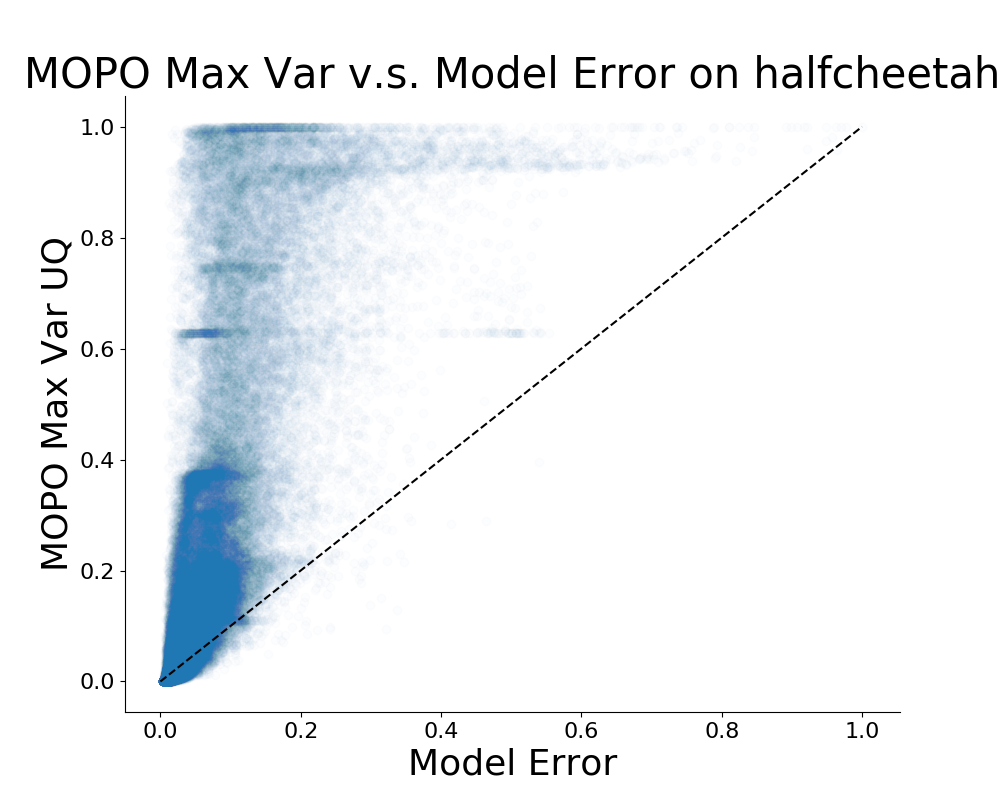
\includegraphics[width=0.47\linewidth]{halfcheetah_medium_corr_var_ood.png}
%     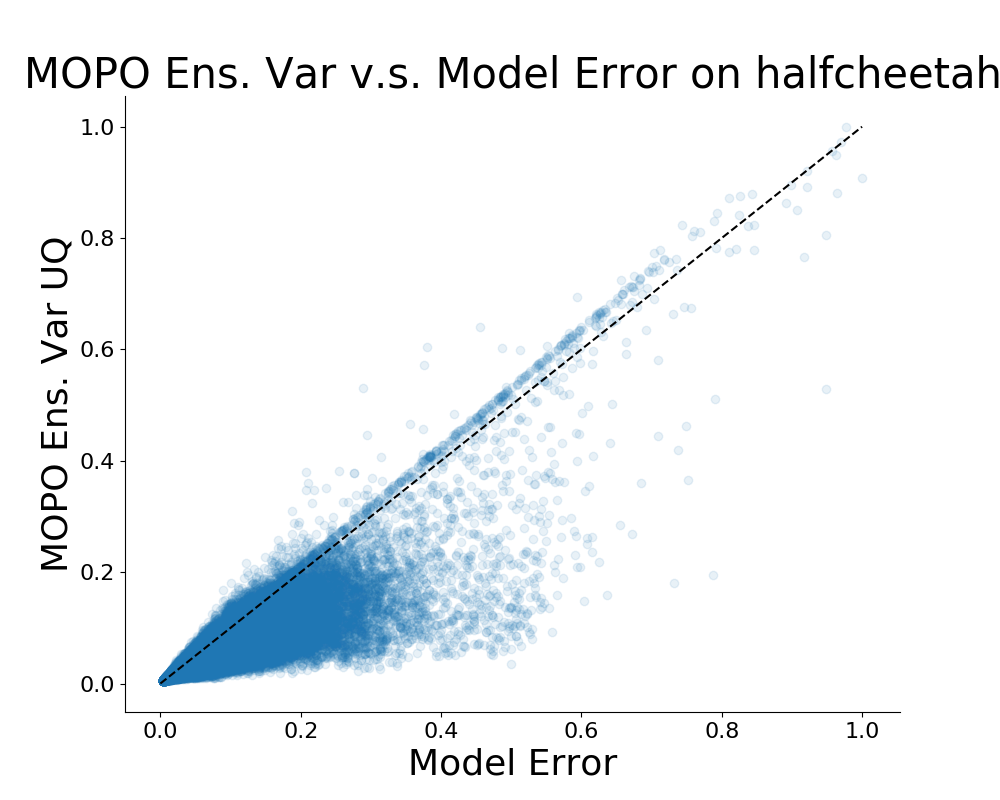
\includegraphics[width=0.47\linewidth]{halfcheetah_medium_corr_lip_ens_ood.png}
%     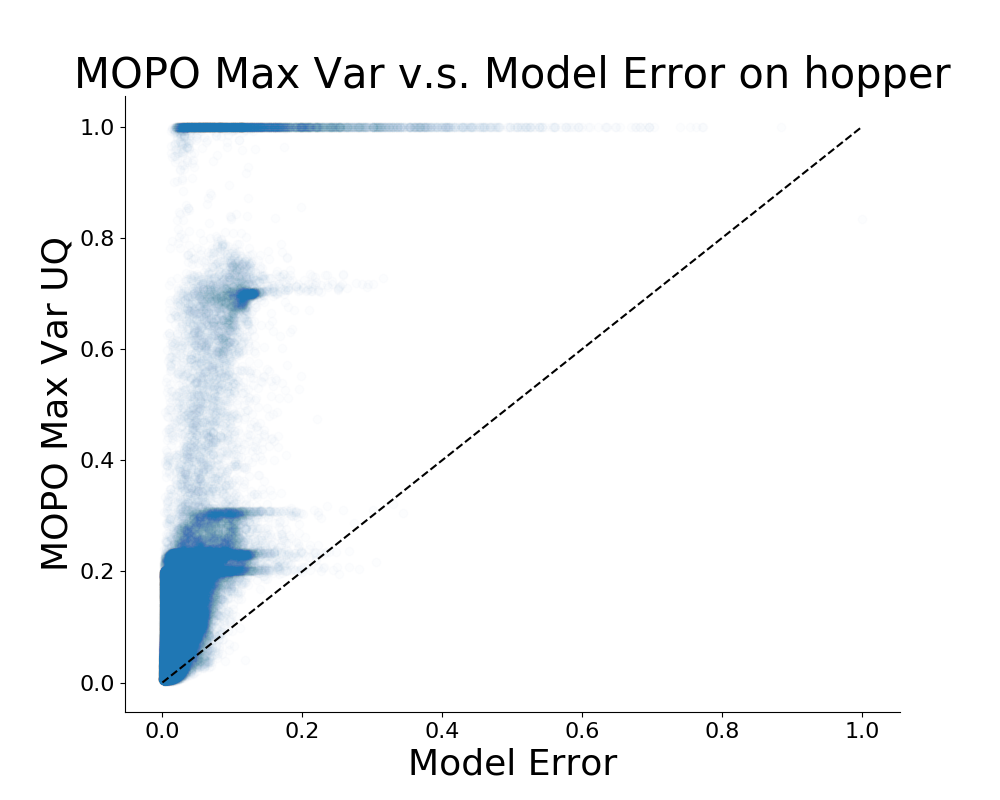
\includegraphics[width=0.47\linewidth]{hopper_medium_corr_var_ood.png}
%     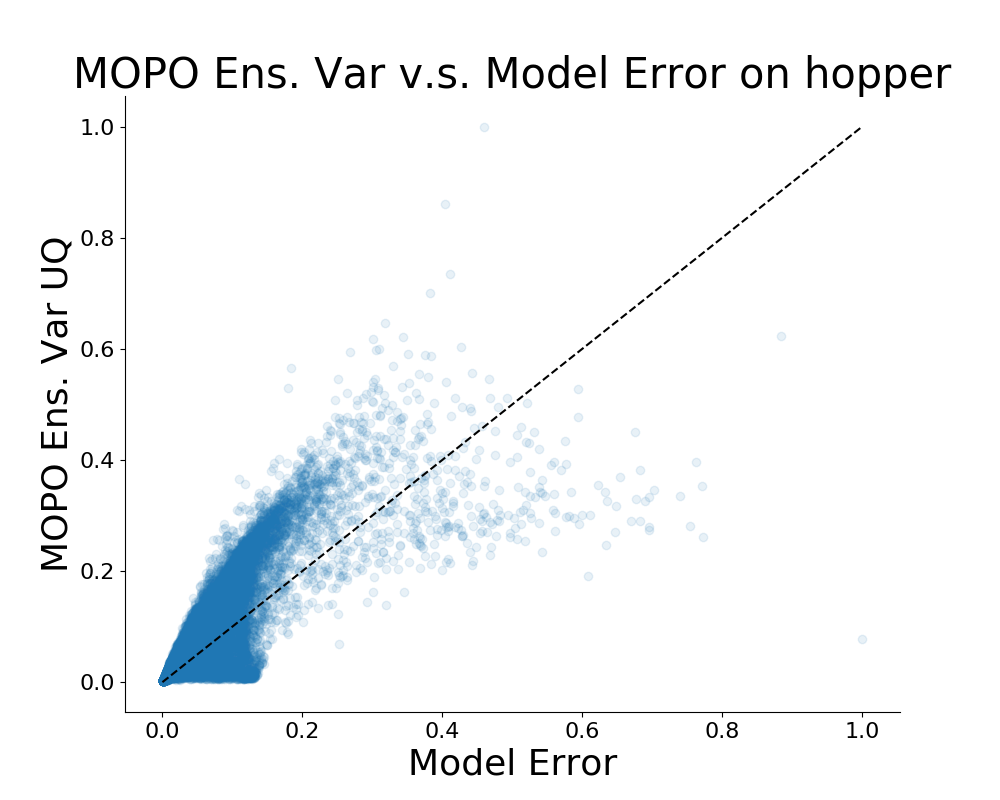
\includegraphics[width=0.47\linewidth]{hopper_medium_corr_lip_ens_ood.png}
%     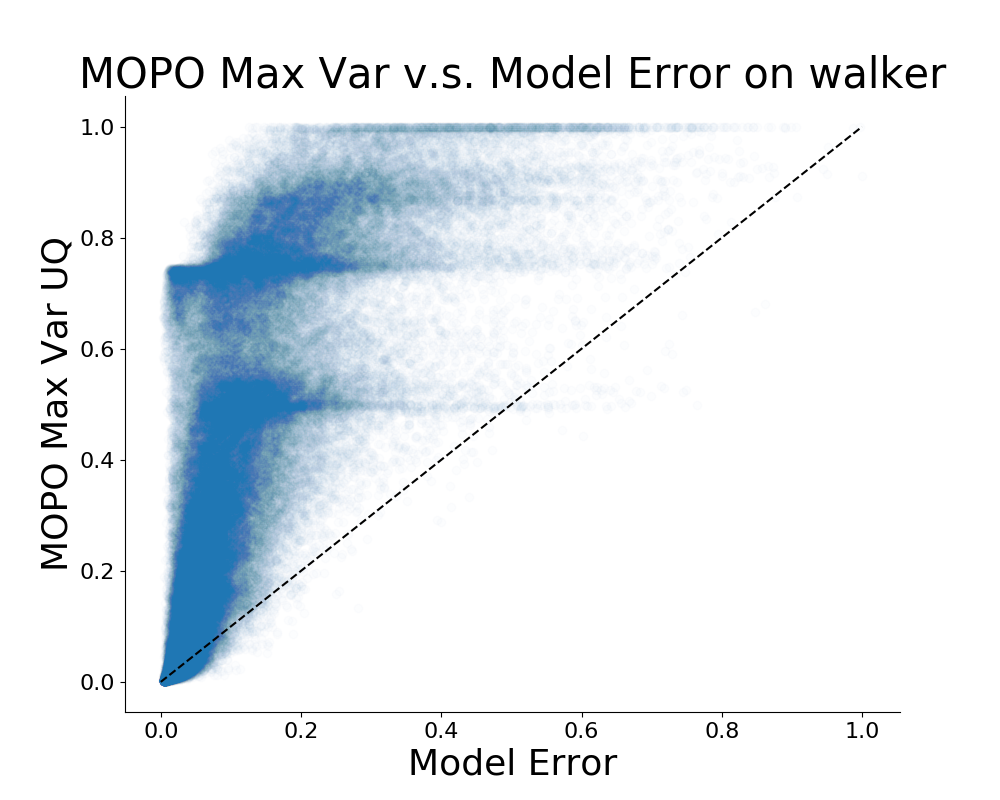
\includegraphics[width=0.47\linewidth]{walker_medium_corr_var_ood.png}
%     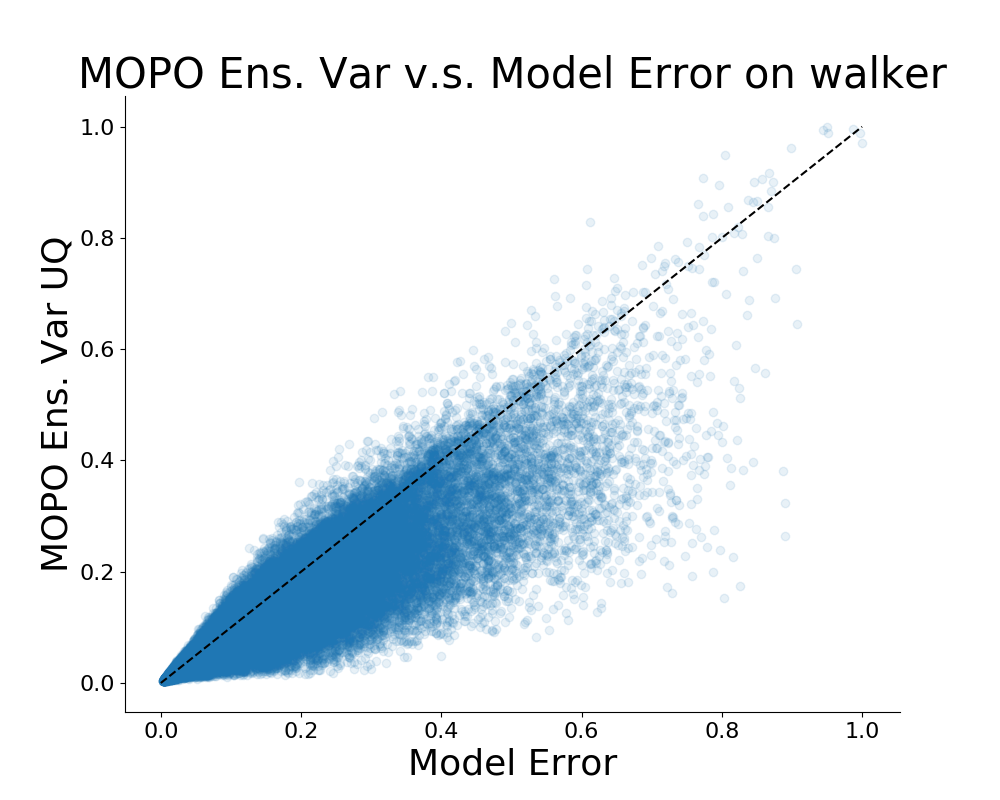
\includegraphics[width=0.47\linewidth]{walker_medium_corr_lip_ens_ood.png}
%     \vspace{-0.2cm}
%     \caption{\footnotesize
%     %
%     We visualize the correlation between the model error and two uncertainty quantification methods maximum learned variance over the ensemble (left column) and variance of the model prediction over the ensemble (right column) on three D4RL medium datasets (from the top row to the bottom row: halfcheetah, hopper and walker) where MOPO performs poorly compared to model-free methods. We show that \textbf{Max Var} tends to be overly conservative and overestimating the model error while \textbf{Ens. Var} is on the opposite. Such visualizations corroborate that uncertainty quantification is challenging with deep neural networks and could lead to poor performance in model-based offline RL. In the meantime, COMBO addresses this issue by removing the burden of performing uncertainty quantification.}
%     \label{fig:uq}
%     \vspace{-0.3cm}
% \end{figure}

% In this section, we perform empirical evaluations to show that uncertainty quantification with deep neural networks, especially in the setting of dynamics model learning, is challenging and could cause problems with uncertainty-based model-based offline RL methods such as MOReL~\citep{kidambi2020morel} and MOPO~\citep{yu2020mopo}. In our evaluations, we consider two uncertainty quantification methods, maximum learned variance over the ensemble (denoted as \textbf{Max Var}) $\max_{i=1,\dots,N}\|\Sigma^i_\theta(\bs,\mathbf{a})\|_\text{F}$ (used in MOPO) and the variance of the model prediction over the ensemble (denoted as \textbf{Ens. Var}) $\max_{i=1,\dots,N}\|\mu^i_\theta(\bs,\mathbf{a}) - \frac{1}{N}\sum_{j=1}^N\mu^j_\theta(\bs,\mathbf{a})\|_2$ (used in MOPO and MOReL) where we use an ensemble of $N$ probabilistic dynamics models $\{\widehat{T}^i_\theta(\bs_{t+1}, r| \bs, \mathbf{a}) = \mathcal{N}(\mu^i_\theta(\bs_t, \mathbf{a}_t), \Sigma^i_\theta(\bs_t, \mathbf{a}_t))\}_{i=1}^N$.

% As shown in Table~\ref{tbl:d4rl}, MOPO performs underwhelmingly on medium datasets in the D4RL datasets where the dataset is collected with a single policy and hence with relatively narrow data coverage of the whole state space. To empirically analyze the poor performance of MOPO on those datasets, we visualize the correlation between the true model error and two uncertainty quantification methods \textbf{Max Var} and \textbf{Ens. Var}. We normalize both the model error and the uncertainty estimates to be within scale $[0, 1]$. As shown in Figure~\ref{fig:uq}, on all three medium datasets, \textbf{Max Var} tends to be overly conservative and \textbf{Ens. Var} behaves too optimistic to correctly quantify the true model error, suggesting that uncertainty estimation used by MOPO is not accurate and might be the major factor that results in its poor performance. Meanwhile, COMBO circumvents challenging uncertainty quantification problem and achieves much better performances on those medium datasets, indicating the effectiveness and the robustness of the method.